% The MACE architecture acts as the inspiration for our contribution. MACE can be split up into x main steps: 

% \begin{enumerate}
%     \item for a given node, form the two-body (i.e. edge) basis states, $\phi$, by projecting the node features onto a set of Moment-Generating Functions (MGFs), these can be of different tensor rank and are split up into an angular part and a radial part.
%     \item for the neighbourhood aggregate all the two-body basis states of the same tensor rank - this is the atomic basis $A_{i,c} = \sum_{j \in \mathcal N(i)} \phi_{j,c}$
%     \item For a given node, take the atomic basis and iterate over the correlation order, $\nu$, from $0 \rightarrow \nu_\text{max}$. $\nu$ tells us the number of terms in the tensor product. We find all possible combinations of terms in this tensor product i.e. A's from a single node of different ranks (each rank can appear once, many times, or not at all). The rank of each tensor product is the sum of the rank of each term. 
%     \item for each TP we contracted down to all possible desired products, the way we do this depends on the MGFs that we use, for Spherical MGFs (i.e. spherical harmonics) we need to use \textit{Clebsch-Gordan} coefficients, whereas for Cartesian MGFs we can use regular tensor contraction via summing over pairs of indices.  
%     \item Then we put all contractions of each desired order out into \textit{bucket} where we take a linear combination of each path via learned weights.
%     \item These then form the messages with which we take a linear combination alongside a weighted mixing of the feature channels
%     \item needs to include the details about channel mixing two times (?) here. 
% \end{enumerate}

% In ACE, a graph structure is formed letting atoms equal nodes and joining atom within some cutoff distance, $r_c$, with edges. This is used in place of the more natural bonds $\equiv$ edges as this misses out non-bonded atoms that are close and effect each other. For each node, its edges are given particle basis states, with are two-body (central and peripheral node) which are aggregated to form an atomic basis (one per node). These atomic basis states can then be multiplied/tensor producted together $v$ times to give $v+1$-body order terms, which form the basis functions $\mathbf{B}$. Using these basis states as a basis for linear regression has proved very effective and rivalled results of many far more complex architectures \cite{kovacs2021linear}.

The Atomic Cluster Expansion (ACE) \cite{drautz2019atomic} has played a crucial role in developing MLIPs. Whilst architectures like Dimenet explicitly account for high body-order terms (to great computational expense) ACE provides a framework for constructing a complete polynomial basis systematically at constant cost per basis function independent of body-order\cite{dusson2022atomic}. ACE takes advantage of a body-order expansion that implicitly generates higher-order terms MACE then uses channel mixing and learned weights to `pick out' this most important terms, Figure \ref{fig:implicit-high-body} shows this process. The MACE/ACE architecture can be split up into four main parts, we will do this in the most general way that applies to both our Cartesian MACE and the MACE framework.

\subsection{Particle Basis, $\phi$}

The particle basis is a two-body basis created between a central node $i$ and peripheral node $j$ that share an edge, where as in other models edges are shared between nodes within the cutoff distance, i.e. $r_{ij} < r_c$. They are a function of relative position, $r_{ij}$, and the features of the peripheral node $h_{j,k,\ell_1}$. As the use of features is asymmetric $\phi_{ij} \neq \phi_{ji}$.

\begin{figure}[H]
    \centering
    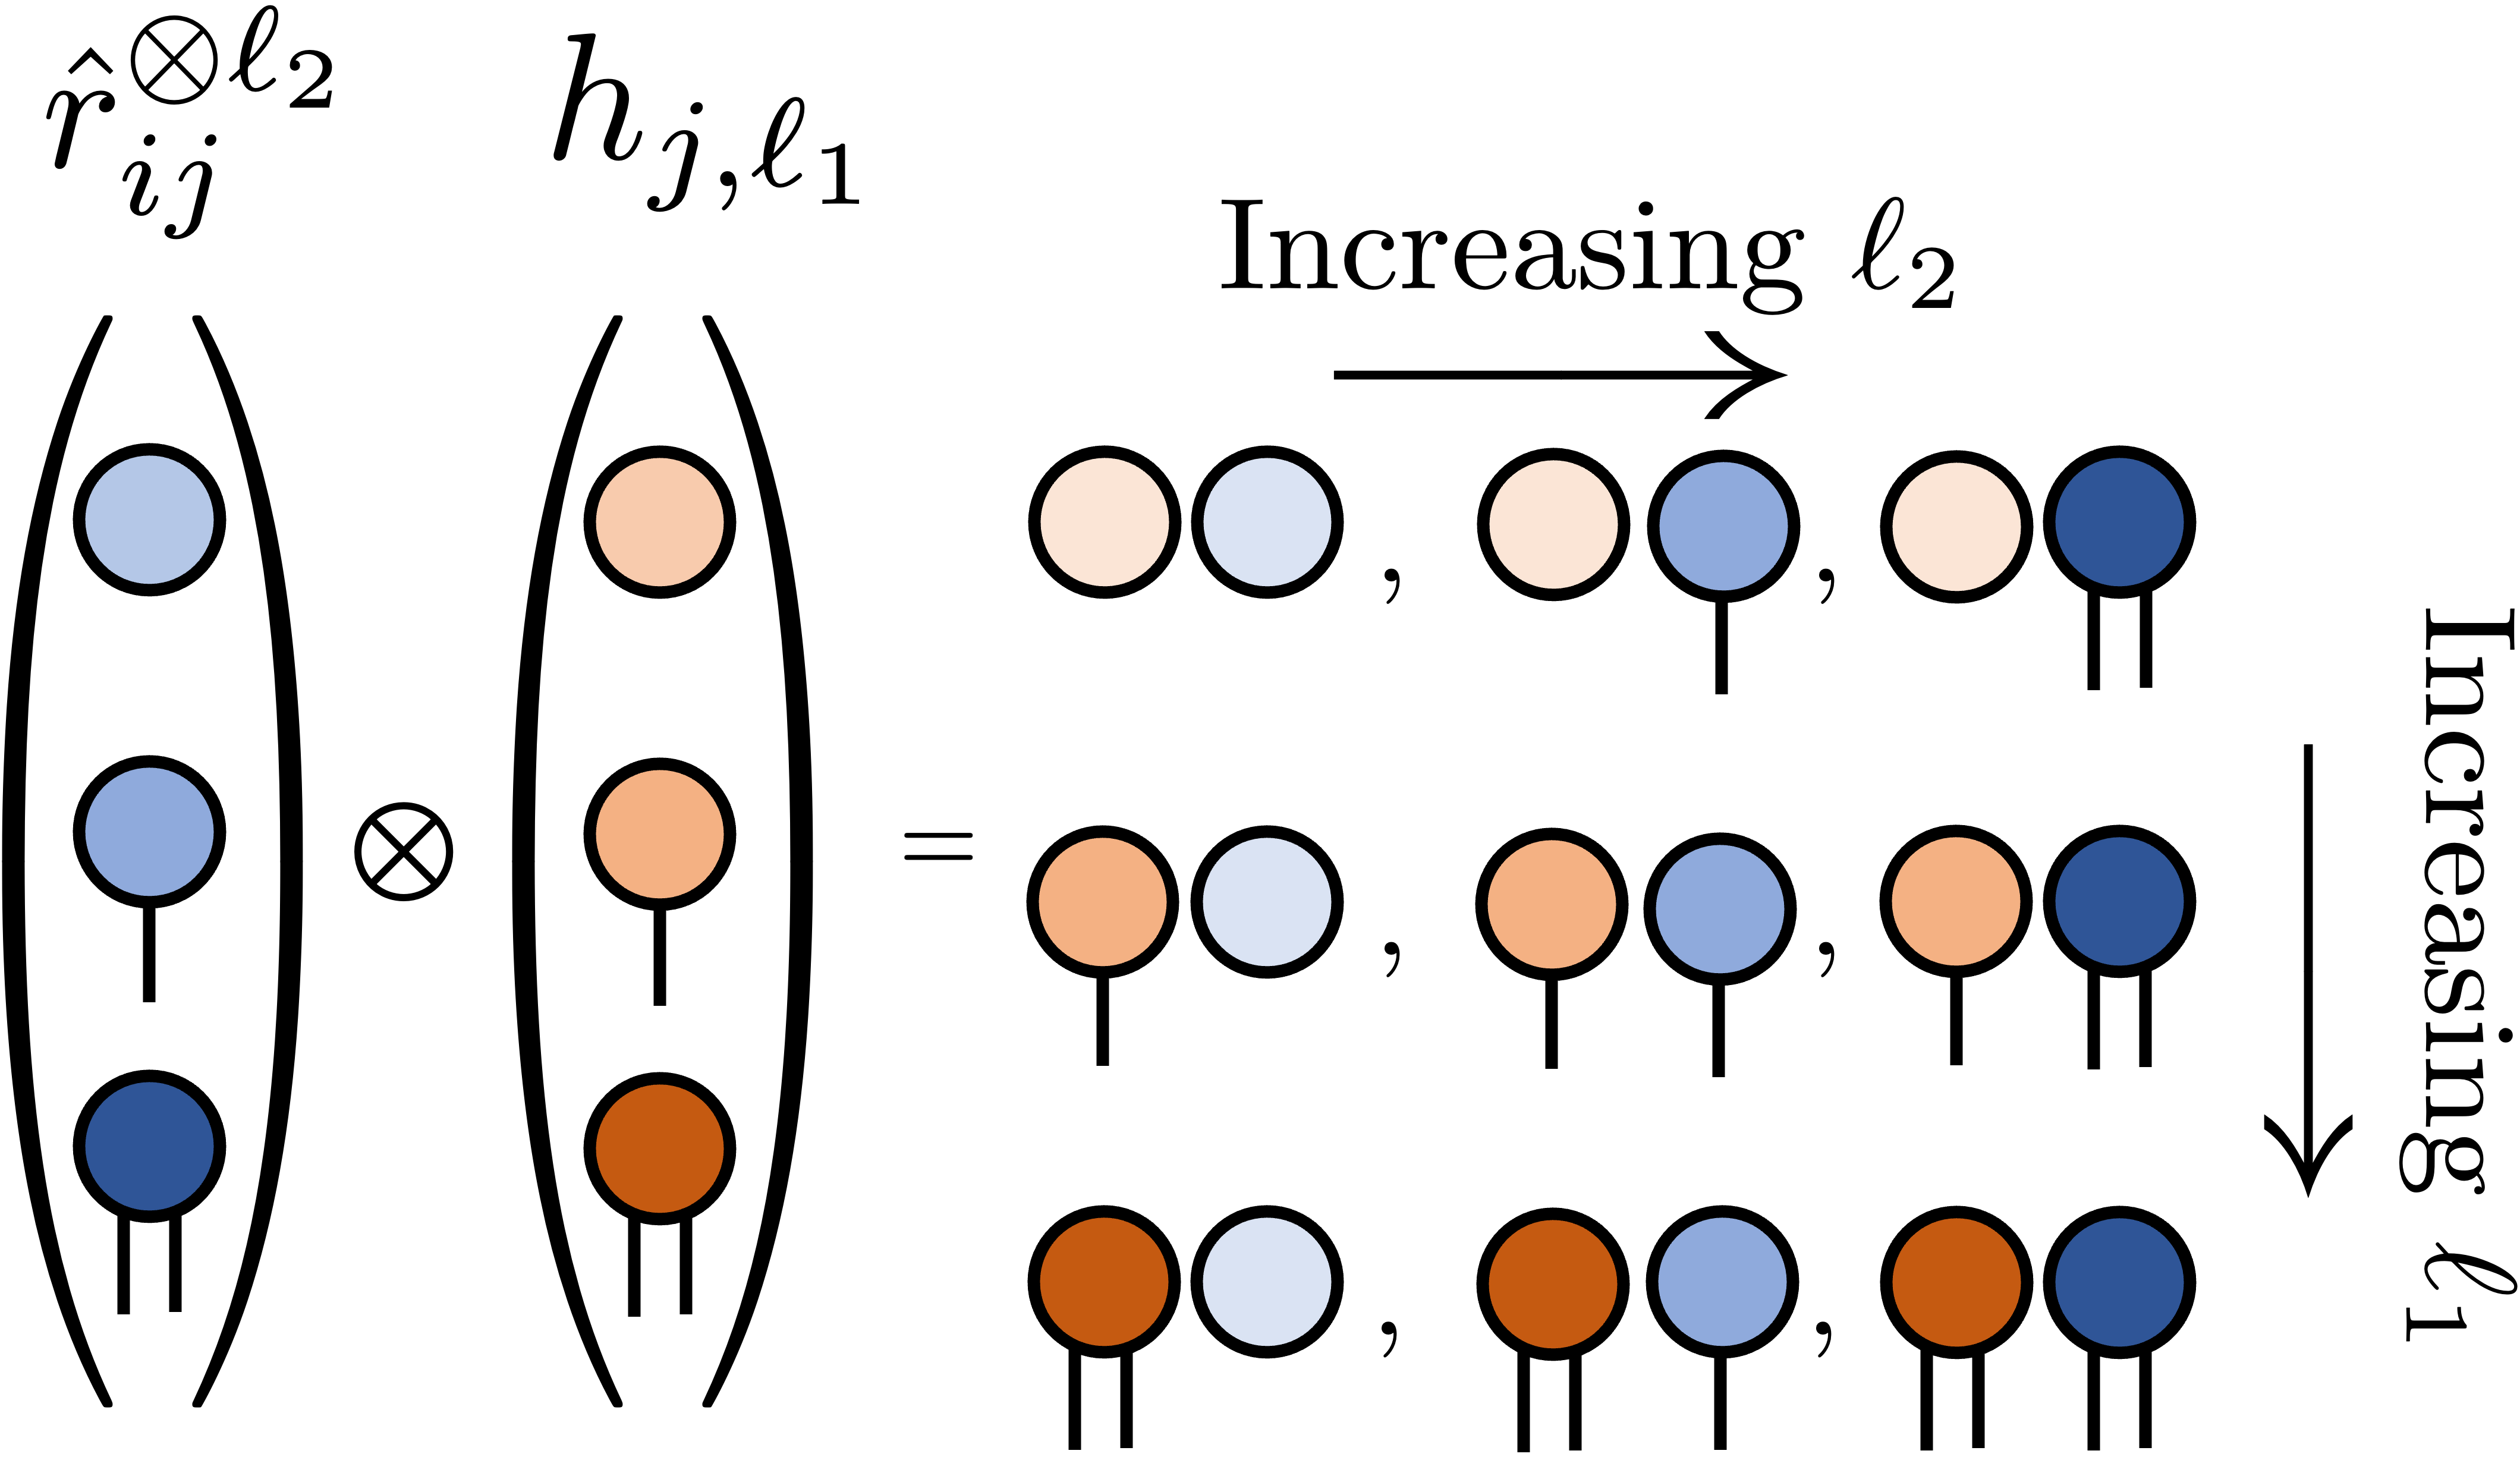
\includegraphics[scale=0.3]{figures/projection.png}
    \caption{The 9 different tensors resulting from the projection of $j$'s feature tensors, with rank-$\ell_1$, onto the angular basis tensors of rank-$\ell_2$. The angular basis is achieve via the outer product of the normalised displacement between $i$ and $j$ $\ell_2$ time. These angular basis functions are inspired by the Moment Tensor Potentials \cite{shapeev2016moment}.}
    \label{fig:projection}
\end{figure}

The particle basis for node $i$ is formed by, first, projecting the channel-mixed features $\texttt{mix}(h_{j,k\ell_1})$ of a neighbouring node $j \in \mathcal N(i)$ of rank-$\ell_1$ onto a set of angular basis tensors, $\Theta_{\ell_2}(\hat r_{ij})$ of rank-$\ell_2$ which are a function of the normalised displacement vector between nodes $i$ and $j$, $\hat r_{ij}$. For MACE these consist of the spherical harmonics $\mathrm Y^m_\ell(\hat r_{ij})$ and for CMACE these are the outer product of the normalised displacement vector, $\hat r_{ij}^{\otimes \ell_2} = \underbrace{\hat r_{ij} \otimes \cdots \otimes \hat r_{ij}}_{\ell_2 \text{times}}$, these are called Moment Tensors \cite{shapeev2016moment}. The projection amounts to a tensor product. This results in tensors with rank-($\ell_1 + \ell_2$), Figure \ref{fig:projection} shows the  $3\times 3 = 9$ projections for when $\ell_1, \ell_2 \in {0,1,2}$. This action is shown in Equation \ref{eq:projection} and produces the intermediate state $\Psi_{ij,k,\ell_1+\ell_2}$.

\begin{equation} \label{eq:projection}
    \Psi_{ij,k,\ell_1+\ell_2} = \Theta_{\ell_2}(\hat r_{ij}) \otimes \texttt{mix}(h_{j,k,\ell_1})
\end{equation}

Next, these projections $\Psi_{ij,k,\ell_1+\ell_2}$ of rank-($\ell_1 + \ell_2$) are contracted to the desired rank $\ell_3$ via the \texttt{contract} operator. Figure \ref{fig:contraction-op} shows how the \texttt{contract} operator gives all possible contraction combinations as a list. In the case of the particle basis we sum up all these different paths and multiply by a scalar radial basis functions (RBFs), $\mathrm R_{k,\ell_1\ell_2\ell_3}(|r_{ij}|)$, which is a function of distance between a node $i$ and its neighbour $j$. This operation is shown in Equation \ref{eq:phi}. These states are therefore two-body as they only include information about two nodes $i$ (position) and $j$ (position and features). The RBFs are indexed by $k,\ell_1,\ell_2,\ell_3$ as there are different learned weights for each combination of the indices, $\ell_1,\ell_2,\ell_3$, but the more important thing is that we scale projections by some radially dependent function. 

\begin{equation} \label{eq:phi}
    \phi_{ij,k,\ell_3} = \sum_{\ell_1 ,\ell_2} \mathrm R_{k,\ell_1\ell_2\ell_3}(|r_{ij}|)\;\underset{\ell_1+\ell_2 \rightarrow \ell_3}{\texttt{contract}}(\Psi_{ij,k,\ell_1+\ell_2})
\end{equation}

\begin{figure}
    \centering
    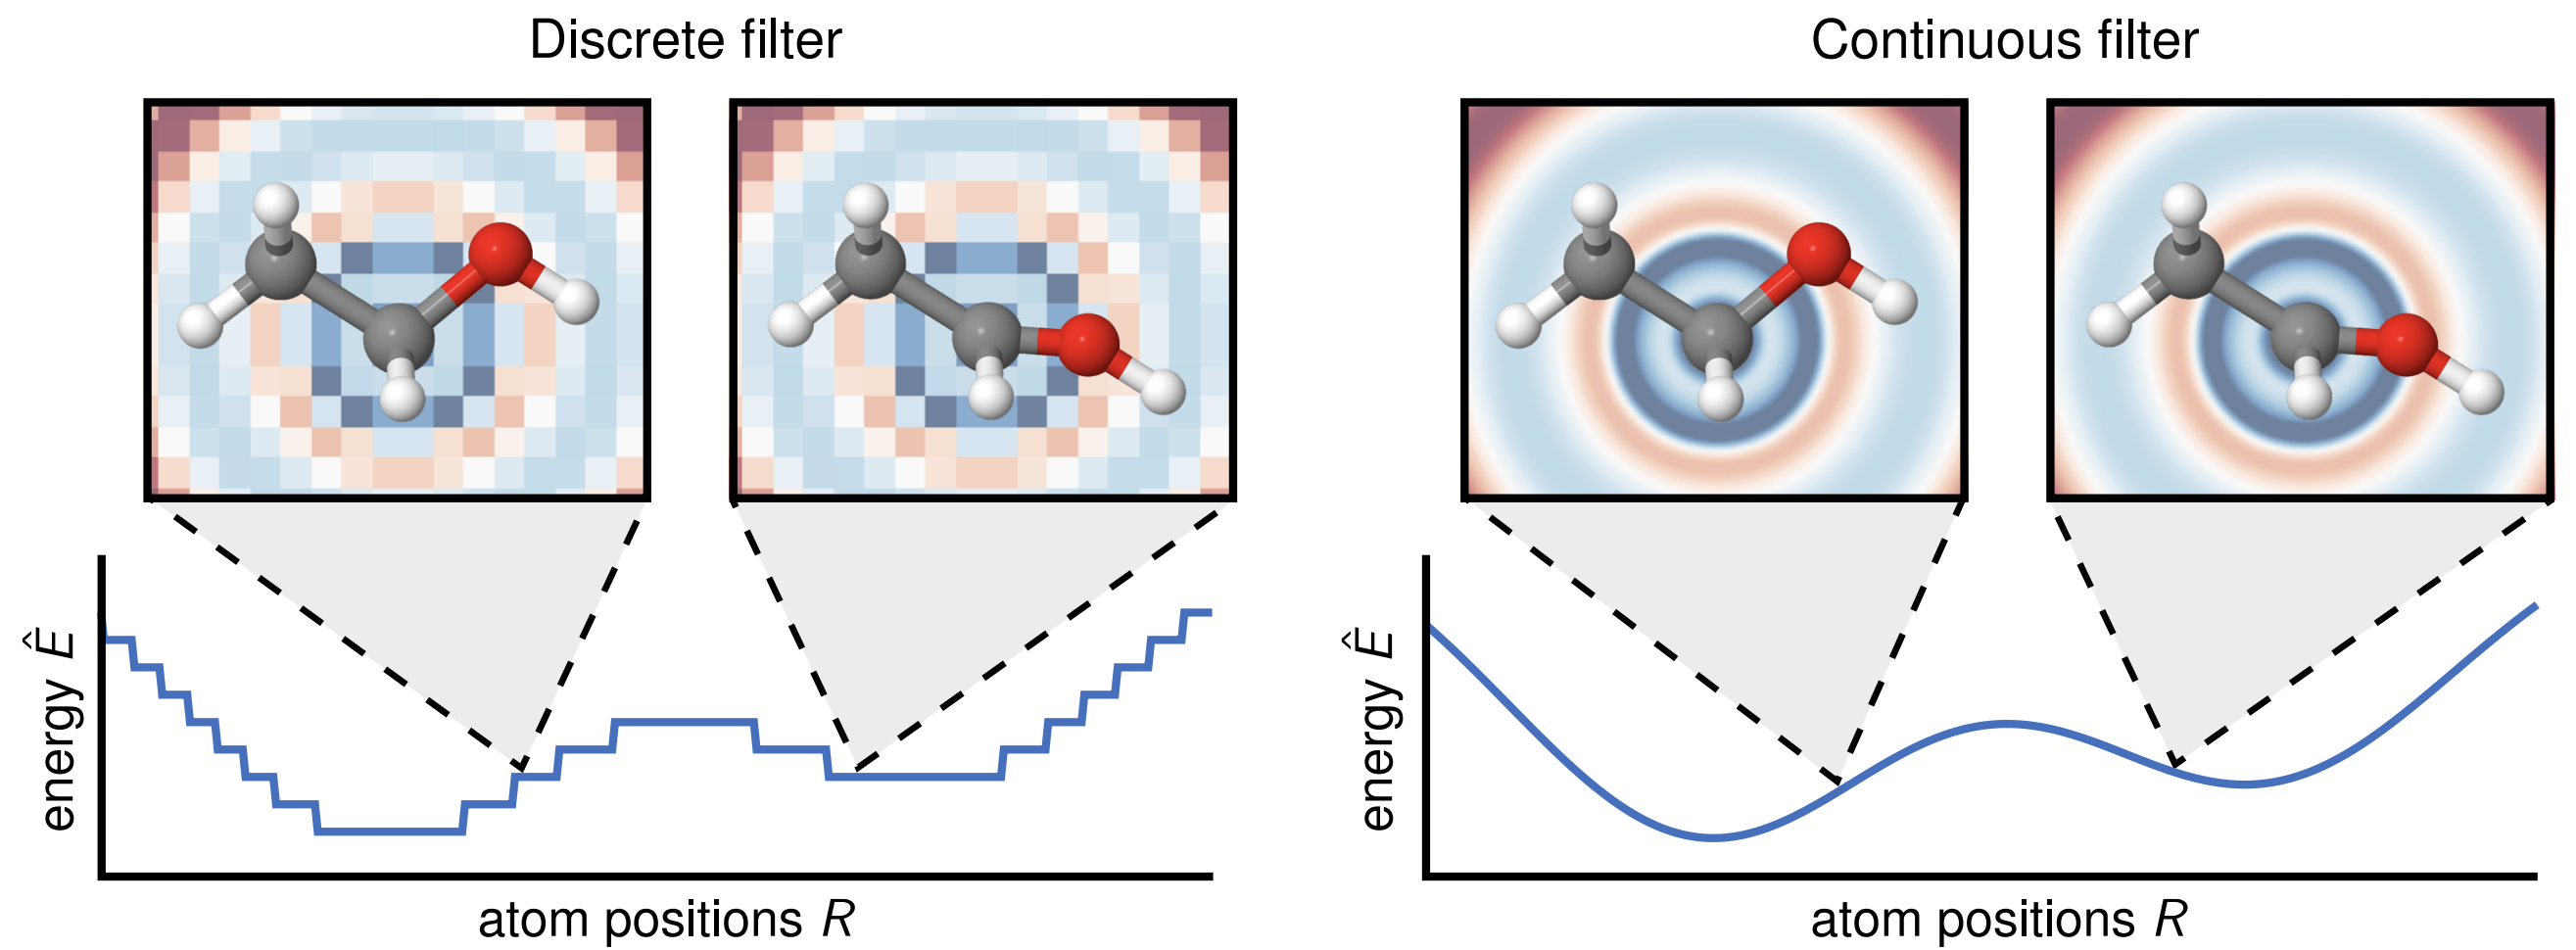
\includegraphics[width=0.7\textwidth]{figures/disc-cont-filter.png}
    \caption{Schnet introduced the idea of smooth radial basis function. This provided smooth output making gradient descent easier}
    \label{fig:disc-cont-filter}
\end{figure}

In the first geometric GNNs \cite{gilmer2017neural} the value of these RBFs were discretised by dividing the distances into bins and assigning values to each of these bins. Schnet was the first model to propose the use of continuous RBFs, this was an essential leap forwards as no only were its outputs continuous and were therefore more physical (see Figure \ref{fig:disc-cont-filter}), this continuity propagates to the loss such that it has a continuous gradient which is essential for gradient descent. Equation \ref{eq:rbf} shows the `Radial Bessel Basis' used by MACE/CMACE as introduced by Dimenet, the frequency grows with the channel number. This physically inspired solution gives an orthogonal set and requires $20\times$ fewer RBFs than the equally-spaced Gaussians used in Schnet.

\begin{equation} \label{eq:rbf}
    R_{\ell_1\ell_2\ell_3,k} (r) = w_{\ell_1\ell_2\ell_3} \sqrt{\frac{2}{c}} \frac{\sin(\frac{k\pi}{c}r)}{r}
\end{equation}

\subsection{Atomic Basis, $A$} 

Formation of the atomic basis is a simple step in which we sum up the two-body particle basis states of each rank (Equation \ref{eq:atomic-basis}), $\phi_{ij,k,\ell_3}$ of node $i$ with all of its neighbours.

\begin{equation} \label{eq:atomic-basis}
    A^{(t)}_{i,k,\ell_3} = \sum_{j \in \mathcal N(i)} \phi_{ij,k,\ell_3}
\end{equation}

This leave each node with an atomic basis feature for every tensor rank. For example, if the maximum rank of $A$ is two, $[A_{i,k,\ell_3=0},A_{i,k,\ell_3=1},A_{i,k,\ell_3=2}]$. 


\subsection{Product Basis, $\mathbf{B}$}

\begin{figure}[H]
    \centering
    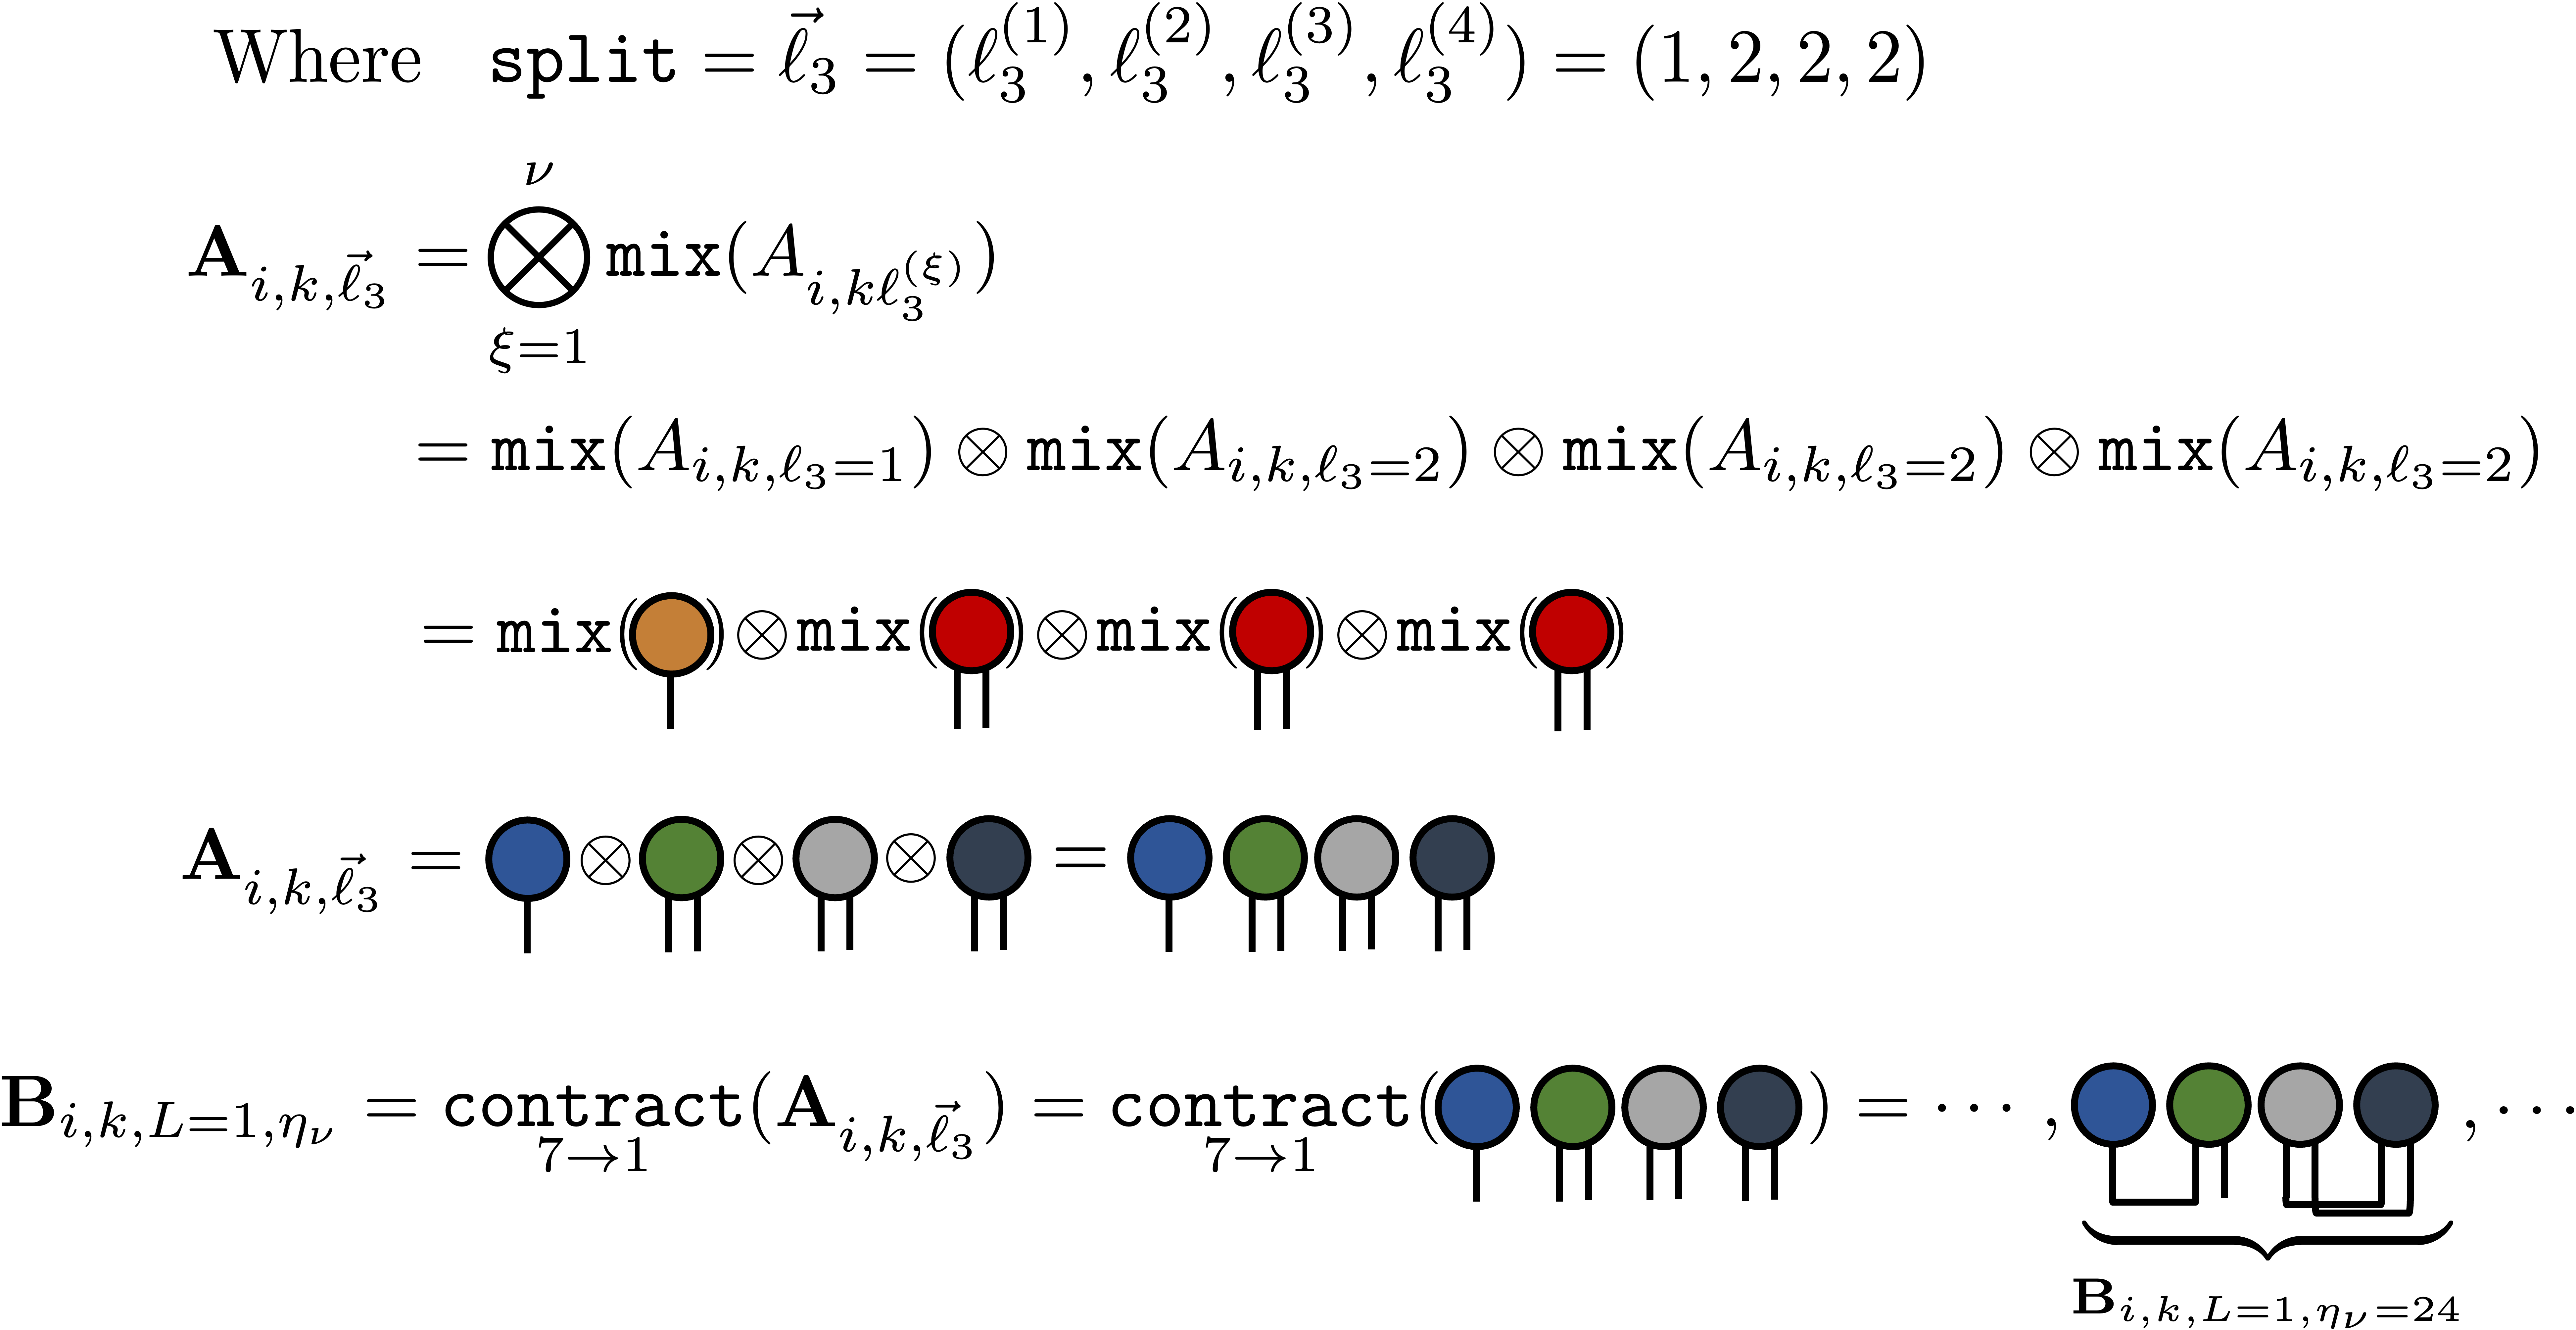
\includegraphics[width=0.8\textwidth]{figures/product-basis.png}
    \caption{process of Equations \ref{eq:product} and \ref{eq:prod-con} turning atomic basis functions for a given node, to the the basis functions $\mathbf B$ for a particular $\texttt{split}=\vec\ell_2 = (1,2,2,2)$ (i.e. one vector and three matrices). The fact all three matrices that are red before the mix are different colours after shows that the weights for each mix is unique. The \texttt{contract} operator is then used as normal.}
    \label{fig:product-basis}
\end{figure}

The formation of the product basis states, $\mathbf{B}$, is the key step that creates implicit higher body-order terms. The $\mathbf B$'s for each node are formed out of only the atomic basis states from that same node. The correlation order, $\nu$ tells us how many different atomic basis tensors will be involved in the creation of a given $\mathbf{B}$.  For each $\nu$ every possible `split' of atomic basis ranks is calculated and denoted by a vector of $\ell_3$'s, $\vec \ell_3$. For example, if $\nu=2$ and the maximum rank of the atomic basis is $2$ we can have six different splits $\vec\ell_3 =(0,0), (0,1), (0,2), (1,1), (1,2), (2,2)$. For each split the $A$'s chosen have their channels mixed (unique to this split). This yields the intermediate tensor representation boldface $\mathbf{A}$ which has the rank $\texttt{sum}(\vec\ell_3)$ which is the sum of elements of $\ell_3$, as seen in its definition in Equation \ref{eq:product}.

\begin{equation} \label{eq:product}
    \mathbf{A}^{(t)}_{i,k,\vec \ell_3} =  \bigotimes_{\xi=1}^{\nu} \texttt{mix}(A^{(t)}_{i,k\ell_\xi}) \quad \text{where} \quad \vec\ell_3 = (\ell^{(1)}_3,\ell^{(2)}_3, \cdots, \ell^{(\nu)}_3)
\end{equation}

After this, like in the production of the two-body particle basis, the \texttt{contract} operator is used to get $\mathbf B$ of the required rank $L$. Except in this case, we do not sum over the possible input splits and output combinations but except denote each unique contraction path by $\eta_\nu$, this can be seen visually in Figure \ref{fig:product-basis}.

\begin{equation} \label{eq:prod-con}
    \mathbf{B}^{(t)}_{i,k,L,\eta_\nu} = \underset{\texttt{sum}(\vec\ell_3) \rightarrow L}{\texttt{contract}}(\mathbf{A}^{(t)}_{i,k,\vec\ell_3})
\end{equation}

\textbf{Implicit high body-order. } The correlation order, $\nu$, is the number of atomic basis tensors are used in constructing each $\mathbf B$ with that correlation order. Figure \ref{fig:implicit-high-body} shows an example where we only consider scalar two-body particle states, with $\nu=2$, here we see that we have implicit three-body terms. More generally, if the correlation order is $\nu$, the highest body-order terms will be $\nu+1$. 

\begin{figure}[H]
    \centering
    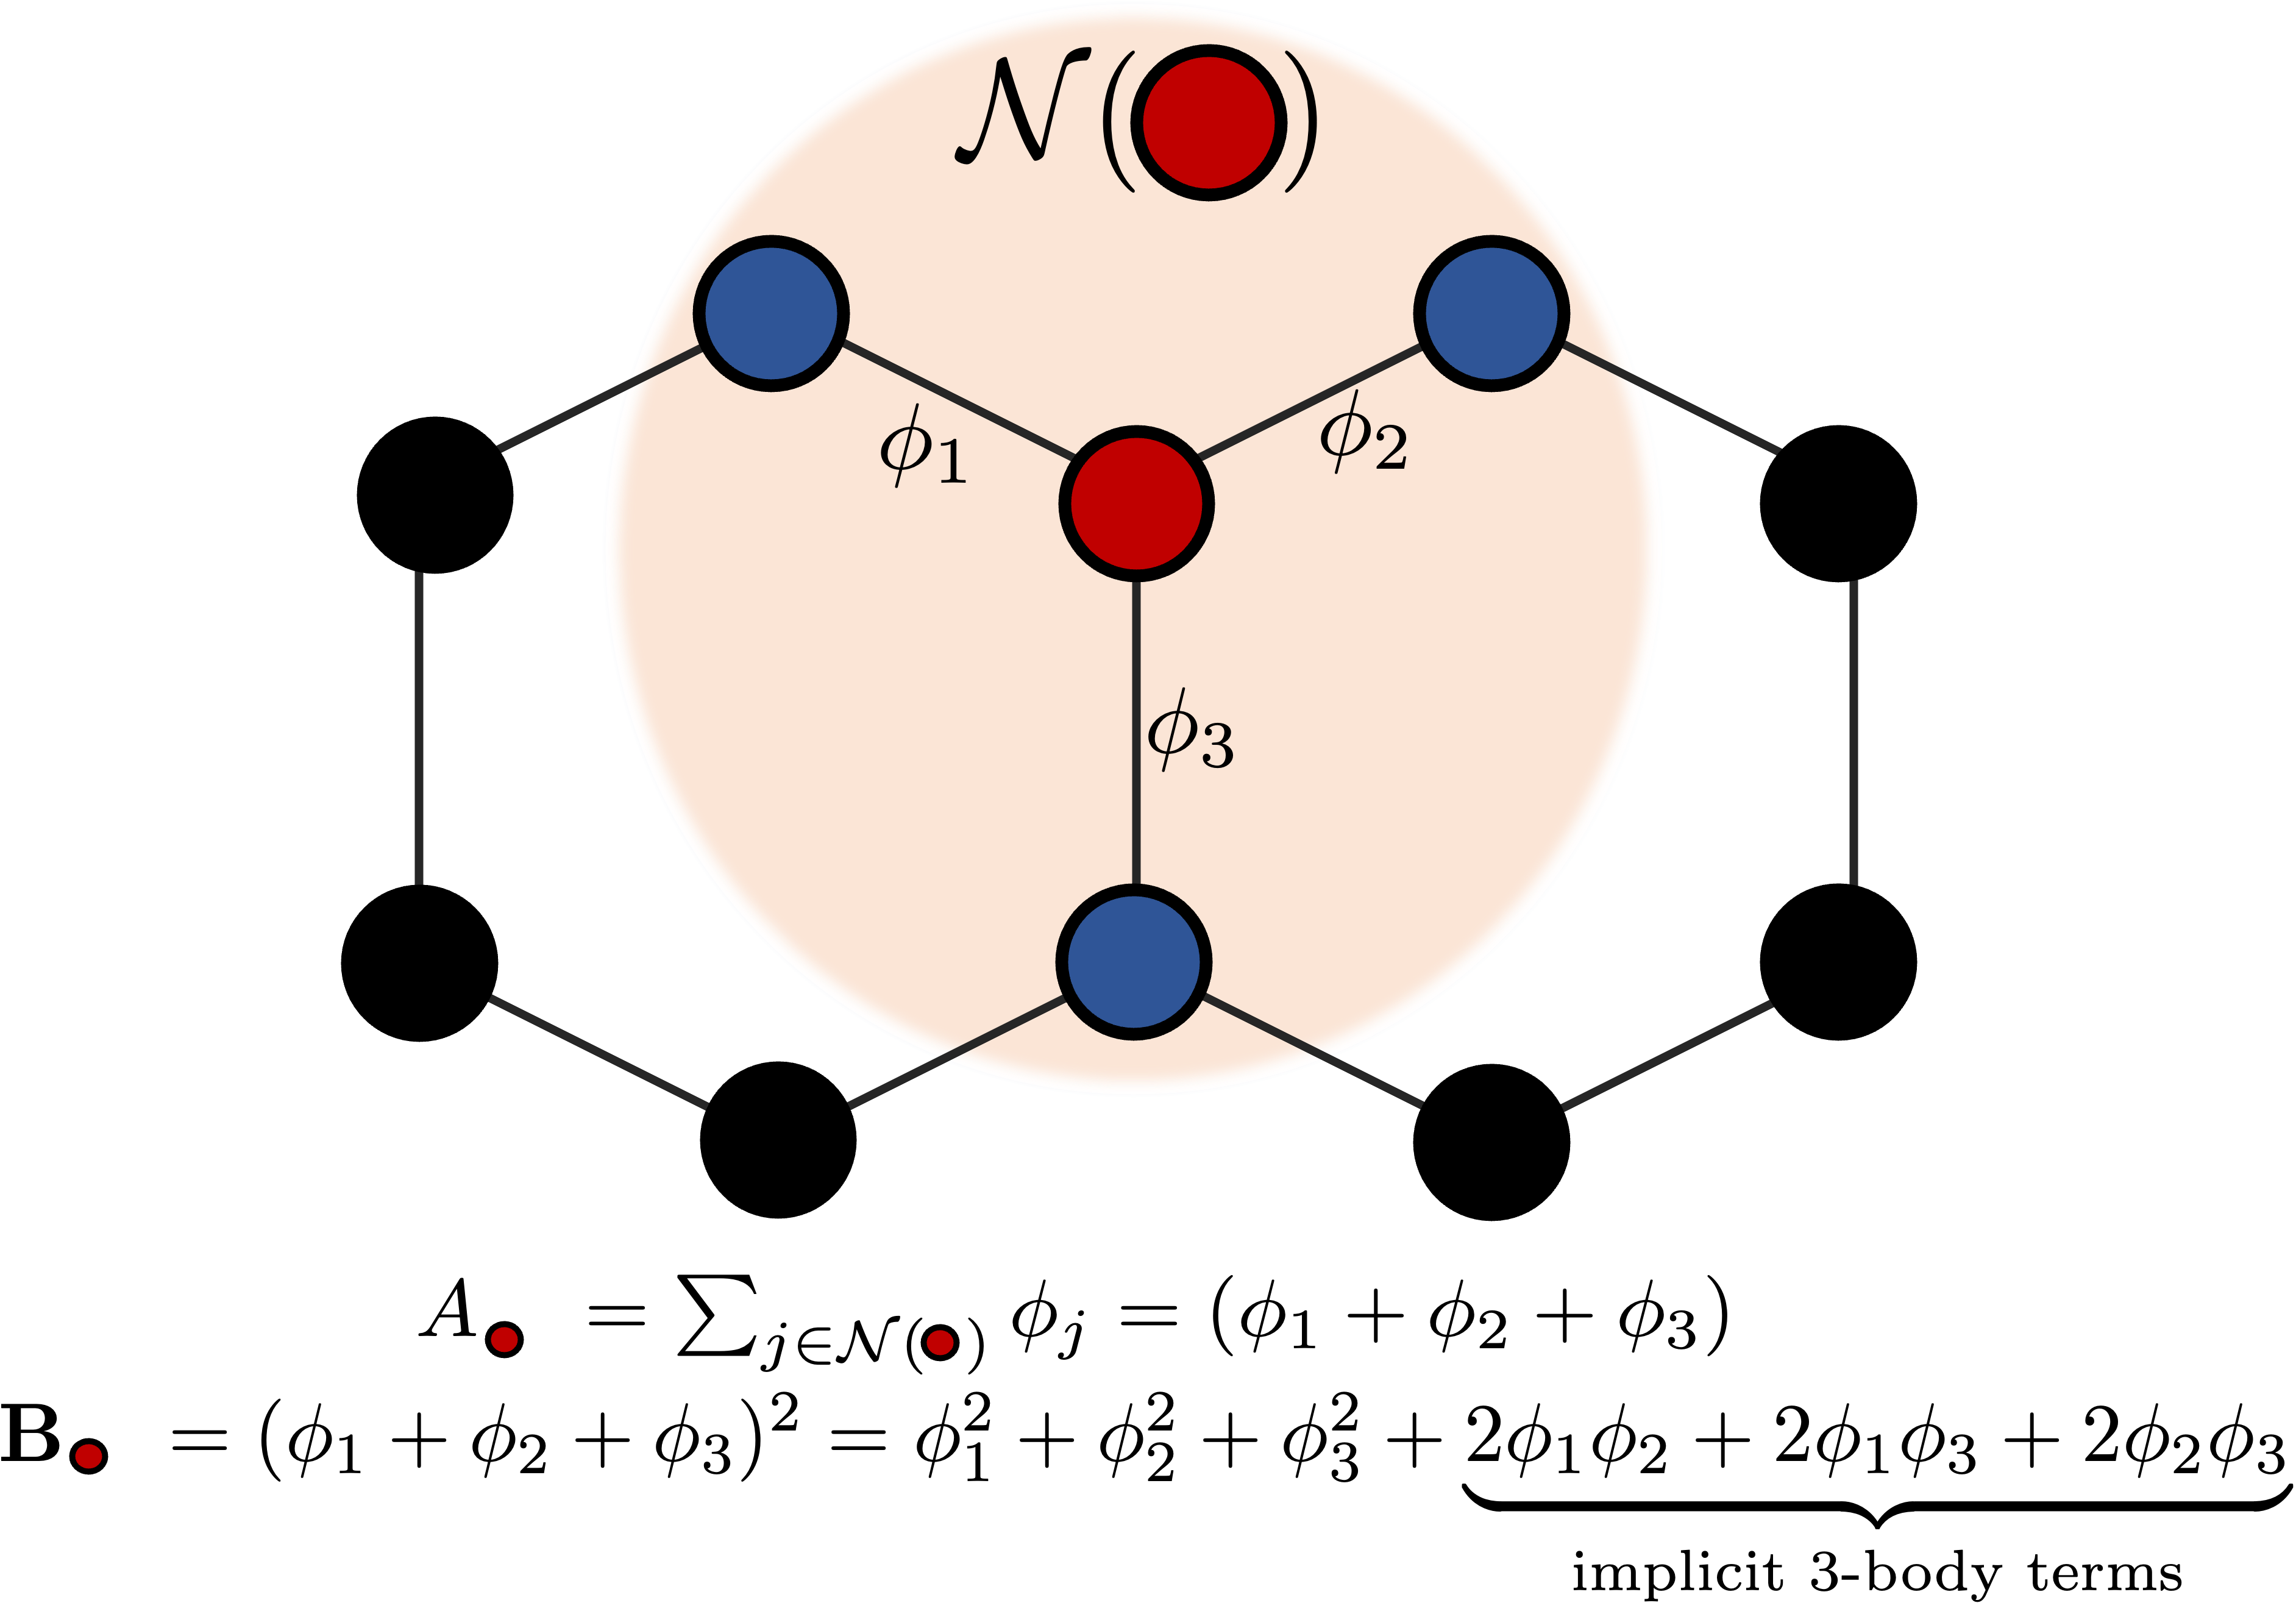
\includegraphics[width=0.7\textwidth]{figures/implicit-high-body.png}
    \caption{This shows how in the neighbourhood of the red node the three particle basis states (which are scalars here for simplicity) with neighbours are aggregated. In this case $\nu=2$ and thus we square the atomic basis states. This gives us terms like $2\phi_1\phi_2$ which are three-body as each particle basis state requires two nodes to make, the central and peripheral.}
    \label{fig:implicit-high-body}
\end{figure}

\textbf{Computational advantage. } The computational speed of MACE comes from the fact that the architecture never explicitly calculates $\mathbf{A}_{i,k,\vec{\ell_3}}$, as the contractions absorb tensor products. For example, if we have two arbitrary tensors $C_{ijk}, D{lmn}$ and carry out the contraction over the indices $(i,l), (j,m), (k,n)$ of the tensor product of $C$ and $D$. Equation \ref{eq:absorb} shows that the order of tensor product vs contraction doesn't matter. 

\begin{equation} \label{eq:absorb}
    \sum_{ijk} E_{ijkijk} = \sum_{ijk} C_{ijk} \otimes D_{ijk}
\end{equation}

The first method needs calculation and storing of tensor $E_{ijklmn}$ with $3^6 = 729$ elements where as the second method need us to access two tensors that are already stored with $2 \times 3^3  = 54$ elements. It is easy to see that this advantage scales exponentially so only becomes more important as the maximum rank of $A$ and $\nu_\text{max}$ grow. 


This process can be conceptualised as extracting low-rank properties of the a high rank tensor (that is never actually calculated). Through the use of learned weights, the most important low-rank properties i.e. $B$'s will becomes very important in the output. This idea is reminiscent of \textit{the kernel trick} used for Support Vector Machines in which a high-dimensional space is implicitly accessed via inner products.

\subsection{The Message, $m$} 

\begin{equation} \label{eq:message}
    m_{i,L}^{(t)} =  \sum^{\nu_\text{max}}_{\nu=1} \sum_{\eta_{\nu}} W_{z_{i} L, \eta_{\nu}}^{(t)} B^{(t)}_{i,\eta_\nu L}
\end{equation}

The \textit{message} is formed via a (learned) linear combination of all the product basis states $B$ (by considering all paths for all correlation order). Figure \ref{fig:create-message} illustrates what this message the scalar and vector message would look like in tensor network notation, with the highest rank representation of the atomic basis being matrices and the maximum correlation order being $4$, the different colours represent channel mixings. 

\begin{figure}[H]
    \centering
    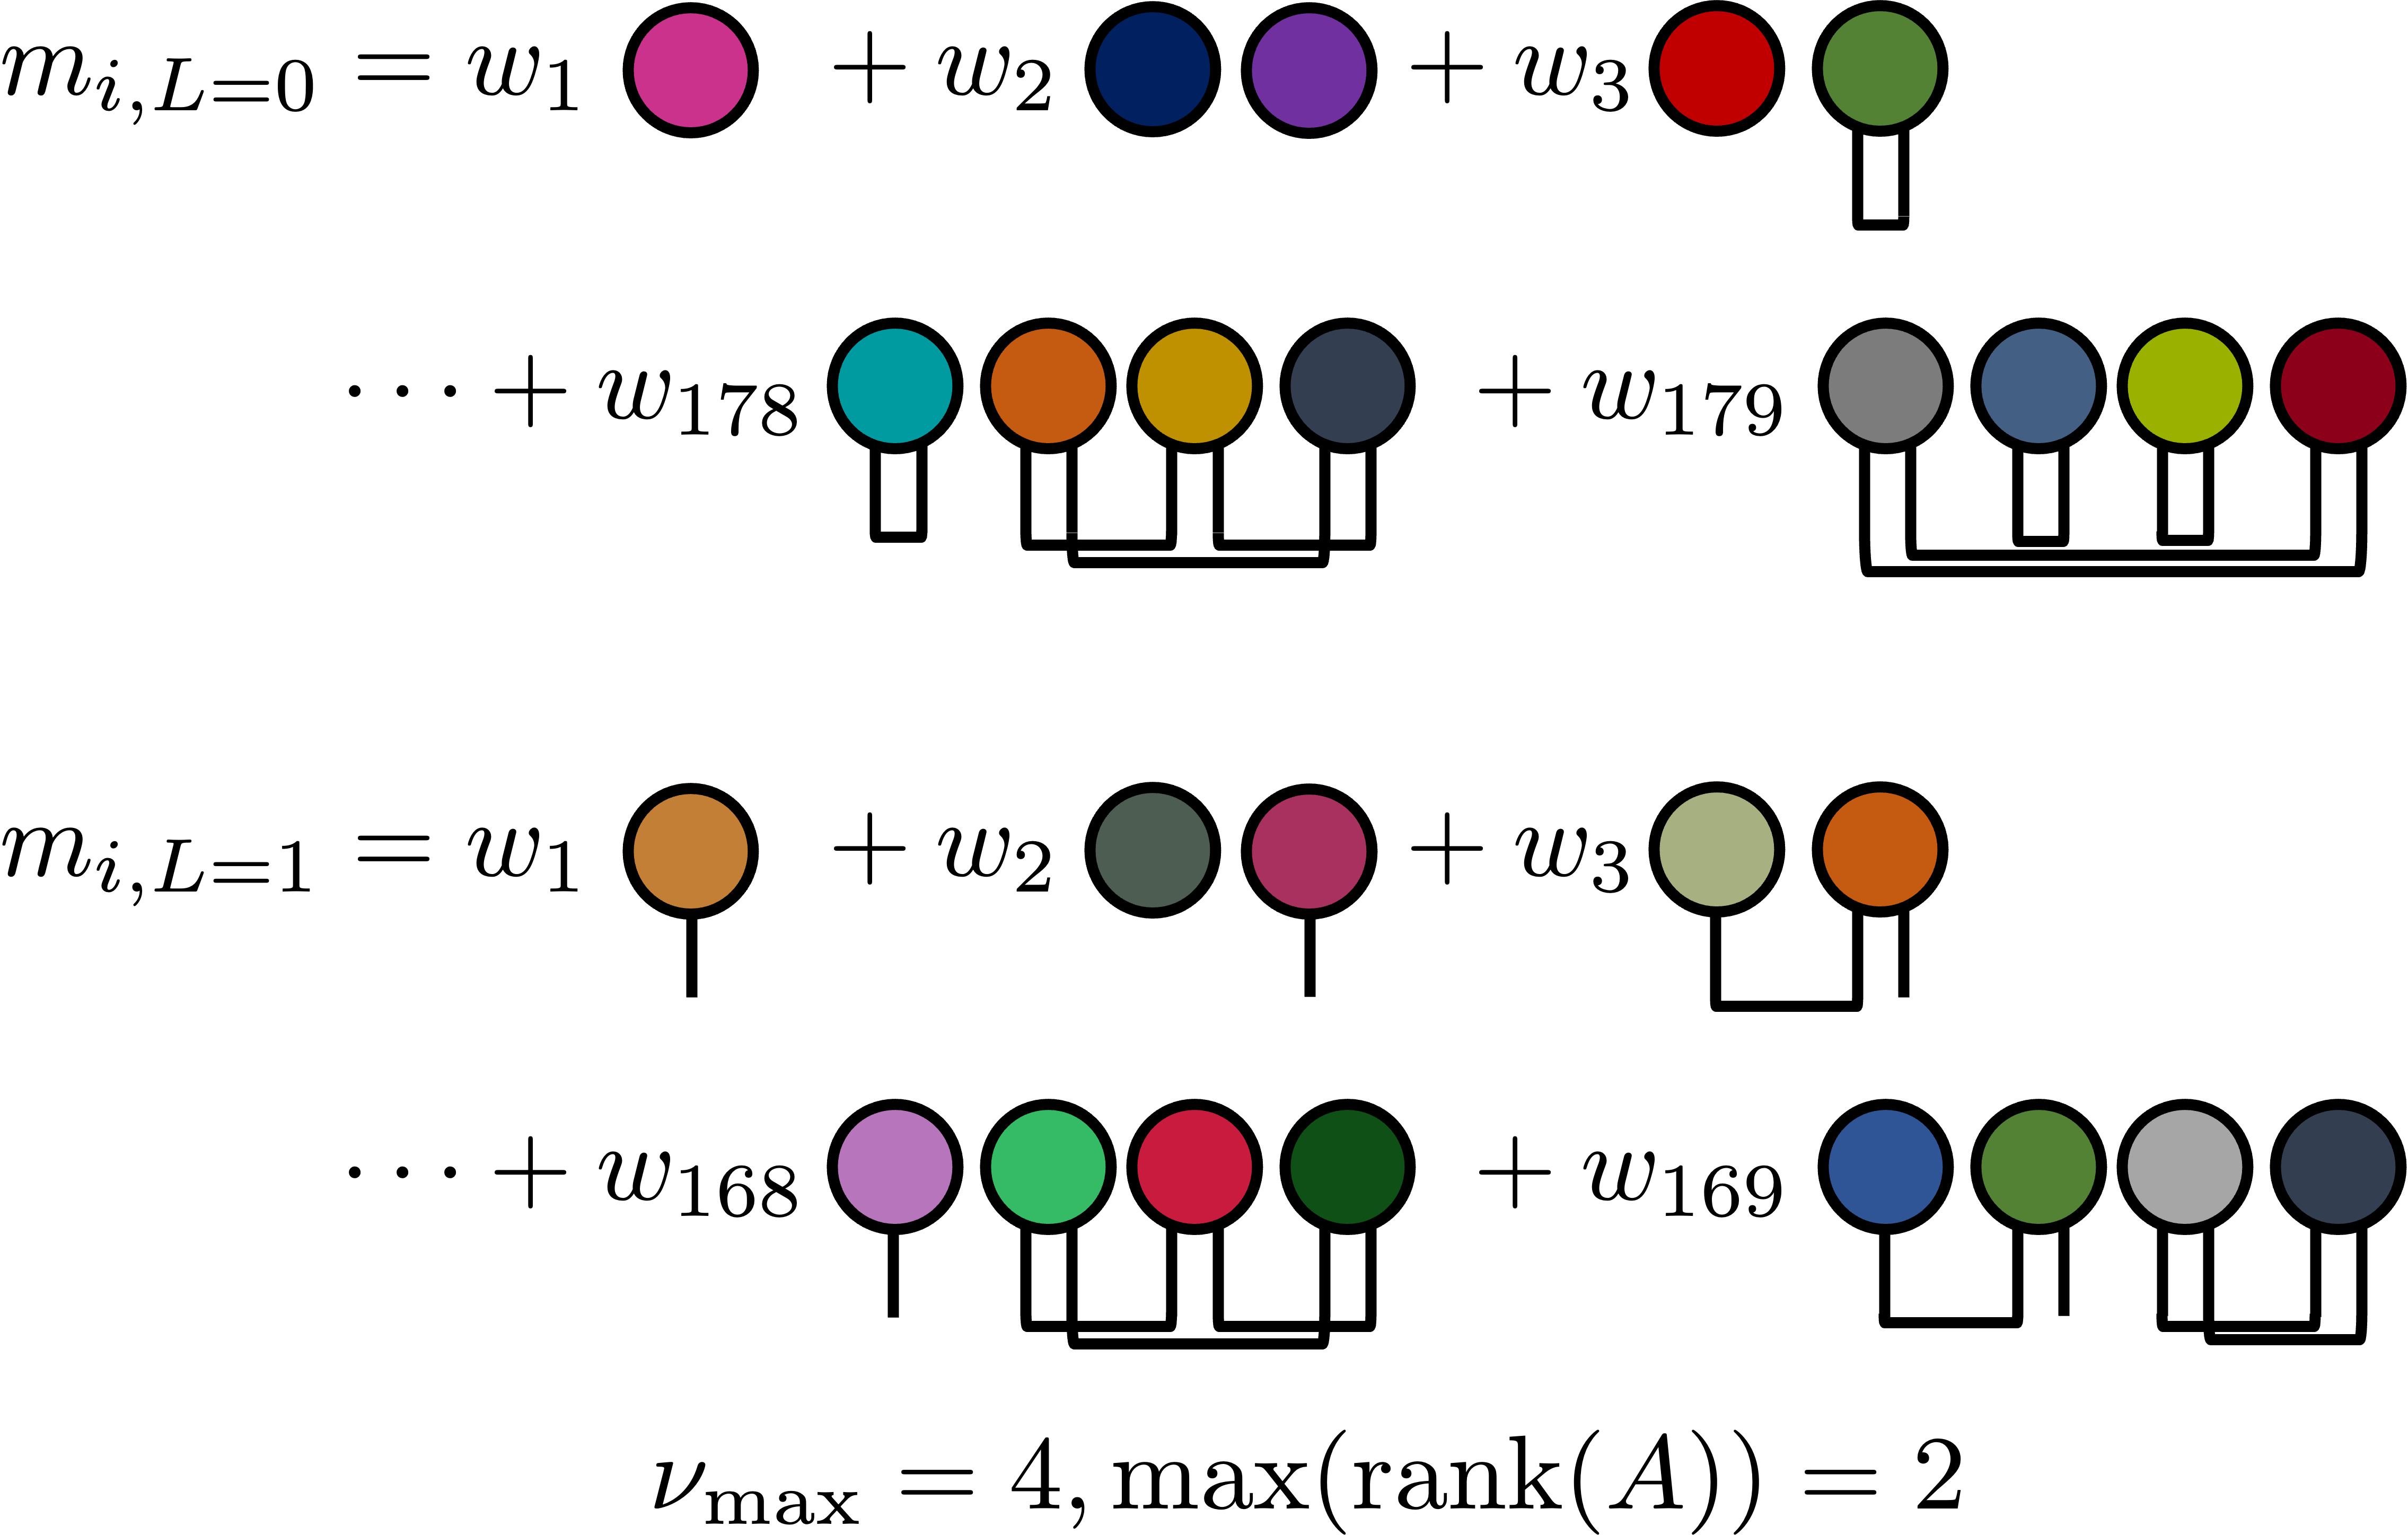
\includegraphics[scale=0.3]{figures/create-message.png}
    \caption{Message creation by a weighted sum of all $\mathbf B$'s of the desired rank. Here we have two examples for $\nu_\text{max}=4$ and maximum atomic basis rank $=2$. Production of scalar and vector messages respectively. $\mathbf B$ with coefficient $w_{169}$ is produced in Figure \ref{fig:product-basis}}
    \label{fig:create-message}
\end{figure}


\subsection{Updating Features} 
Features are then updated via Equation \ref{eq:update} in which the channels of the messages are mixed and are added together with the current features whose channels have also been mixed, this is called a residual connection \cite{he2016deep} which works under the basic principle that to prevent vanishing gradient we should use `skip' connections between layers.  

\begin{equation} \label{eq:update}
    h^{(t+1)}_{i,k L} = \texttt{mix}(m^{(t)}_{i,k, L})
    + \texttt{mix}(h^{(t)}_{i,k,L})
\end{equation}

% \subsection{Particle Basis, $\phi$}

% The particle basis is a two-body basis created between a central node $i$ and peripheral node $j$ that share an edge. They are a function of relative position, $r_{ij}$, and the features of the peripheral node. As the use of features is asymmetric $\phi_{ij} \neq \phi_{ji}$.


% \begin{equation} \label{eq:particle-basis}
%     \phi_{ij,k\ell_3} =  \underset{\ell_1+\ell_2 \rightarrow \ell_3}{\mathrm{contract}} \left[ \mathrm R_{k,\ell_1\ell_2\ell_3}(|r_{ij}|) \Theta_{\ell_2}(\hat r_{ij}) \otimes \mathrm{mix}(h_{j,k\ell_1}) \right]
% \end{equation}

% \begin{figure}[H]
%     \centering
%     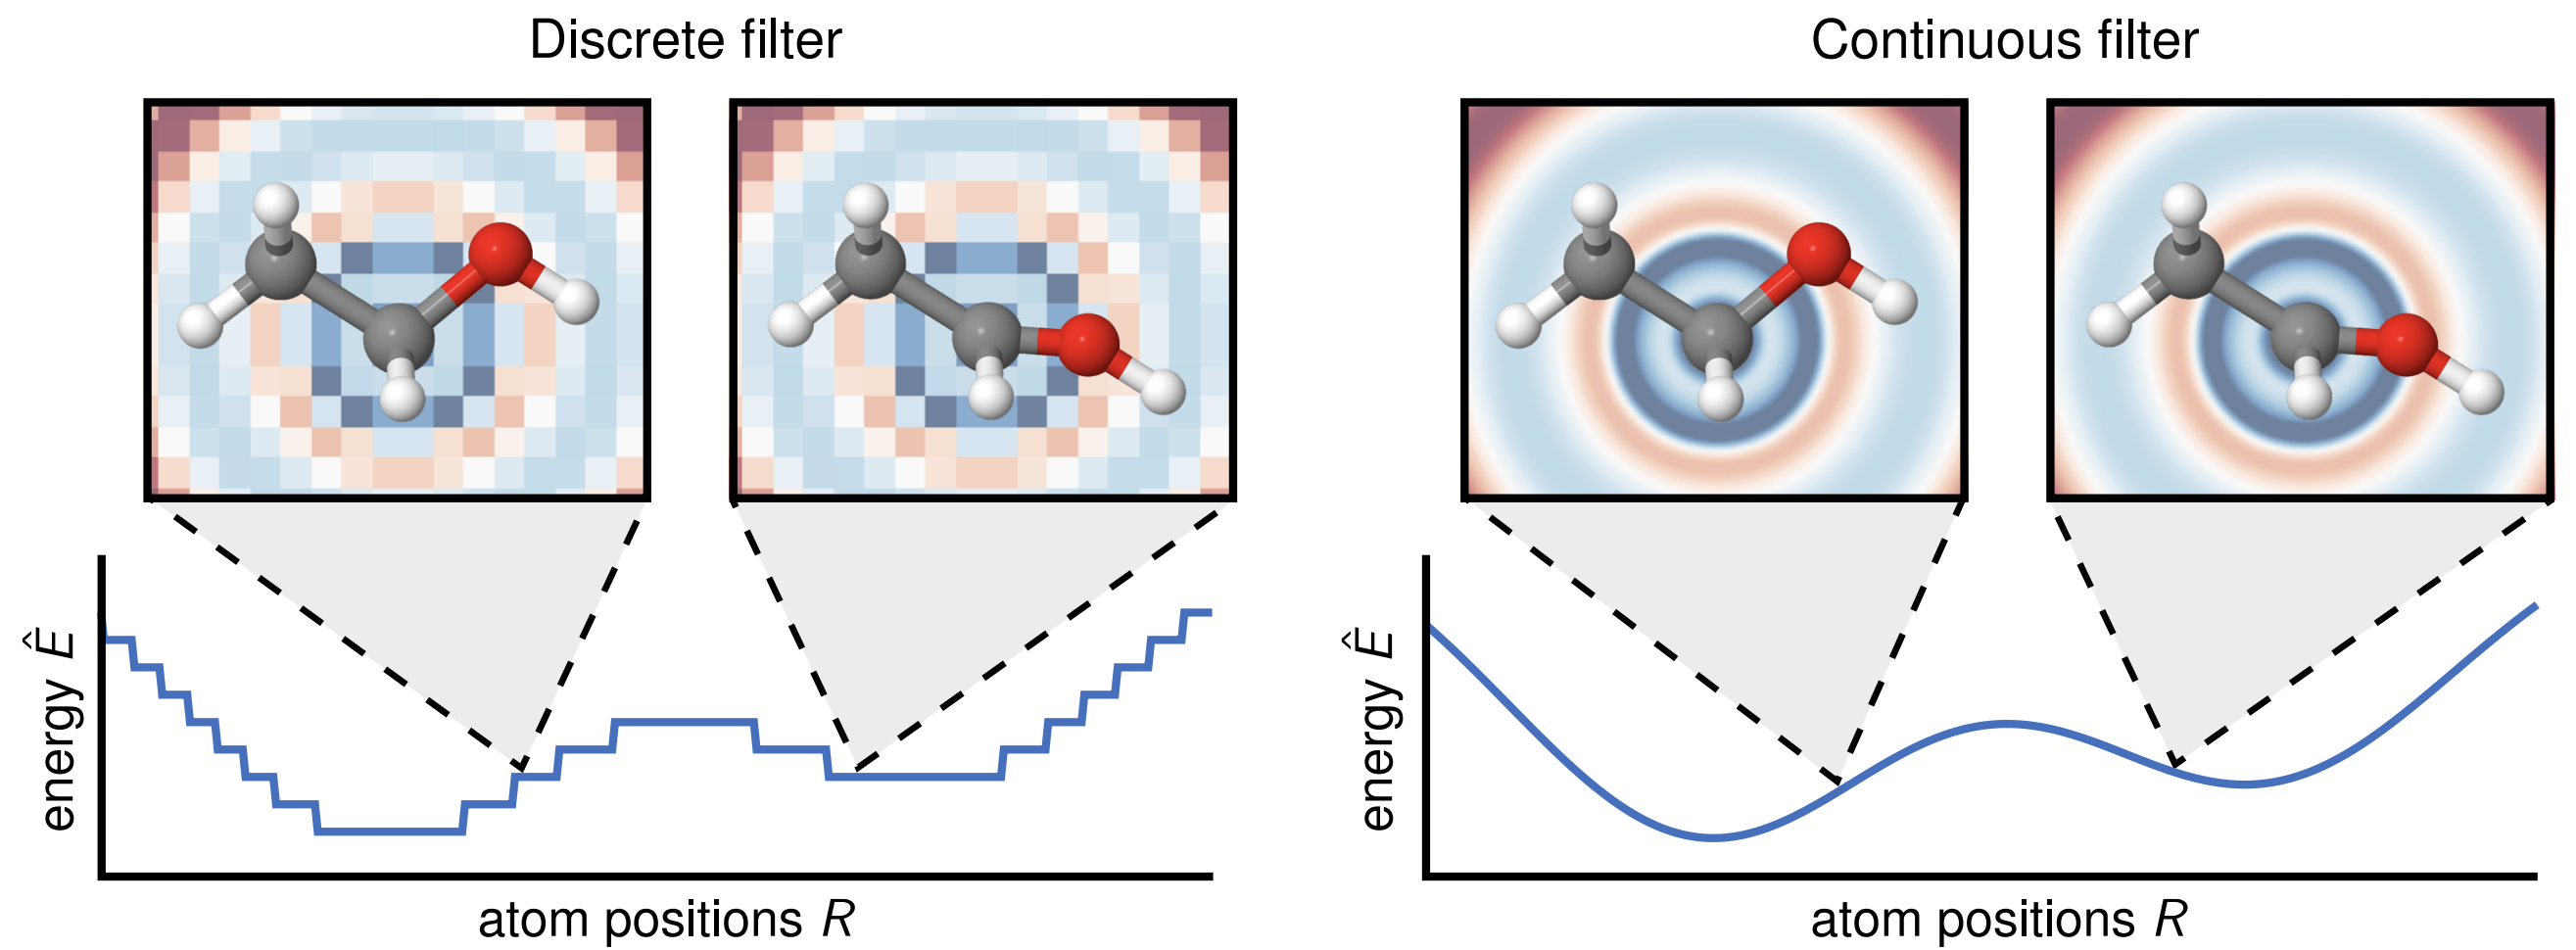
\includegraphics[width=\textwidth]{figures/disc-cont-filter.png}
%     \caption{The use of a continous radial convolution leads to smooth output of network which is more readily differentiable leading to more efficient learning \cite{schutt2017schnet}}
%     \label{fig:disc-cont-filter}
% \end{figure}

% \textbf{Basis functions. } The scalar radial basis functions (RBFs), $\mathrm R_{k,\ell_1\ell_2\ell_3}(|r_{ij}|)$ are a function of the absolute distance between a node $i$ and its neighbour $j$. In the first geoemtric GNNS \cite{gilmer2017neural} the value of these RBFs were discretised by dividing the distances into bins and assigning values to each of these bins. Schnet was the first model to propose the use of continuous RBFs, this was an essential leap forwards as no only were its outputs continuous and were therefore more physical (see Figure \ref{fig:disc-cont-filter}, but this continuity propagates to the loss such that it has a continuous gradient which is essential for learning weights. Equation \ref{eq:rbf} shows the `Radial Bessel Basis' used by MACE/CMACE as introduced by Dimenet, the frequency grows with the channel number. This physically inspired solution gives an orthogonal set and requires 20x fewer RBFs than the equally-spaced Gaussians used in Schnet. The RBFs are indexed by $k,\ell_1,\ell_2,\ell_3$ as there are different learned weights for each combination of the indices, $\ell_1,\ell_2,\ell_3$ and for each channel, $k$

% \begin{equation} \label{eq:rbf}
%     R_{\ell_1\ell_2\ell_3,k} (r) = w_{\ell_1\ell_2\ell_3} \sqrt{\frac{2}{c}} \frac{\sin(\frac{k\pi}{c}r)}{r}
% \end{equation}

% The angular functions, $\Theta_{\ell_2}(\hat r_{ij})$ are a function of the normalised displacement vector between nodes $i$ and $j$. For MACE these consisted of the spherical harmonics $\mathrm Y^m_\ell(\hat r_{ij})$ and for CMACE these were the outer product of the normalised displacement vector, $\hat r_{ij}^{\otimes \ell}$.

% \begin{figure}[H]
%     \centering
%     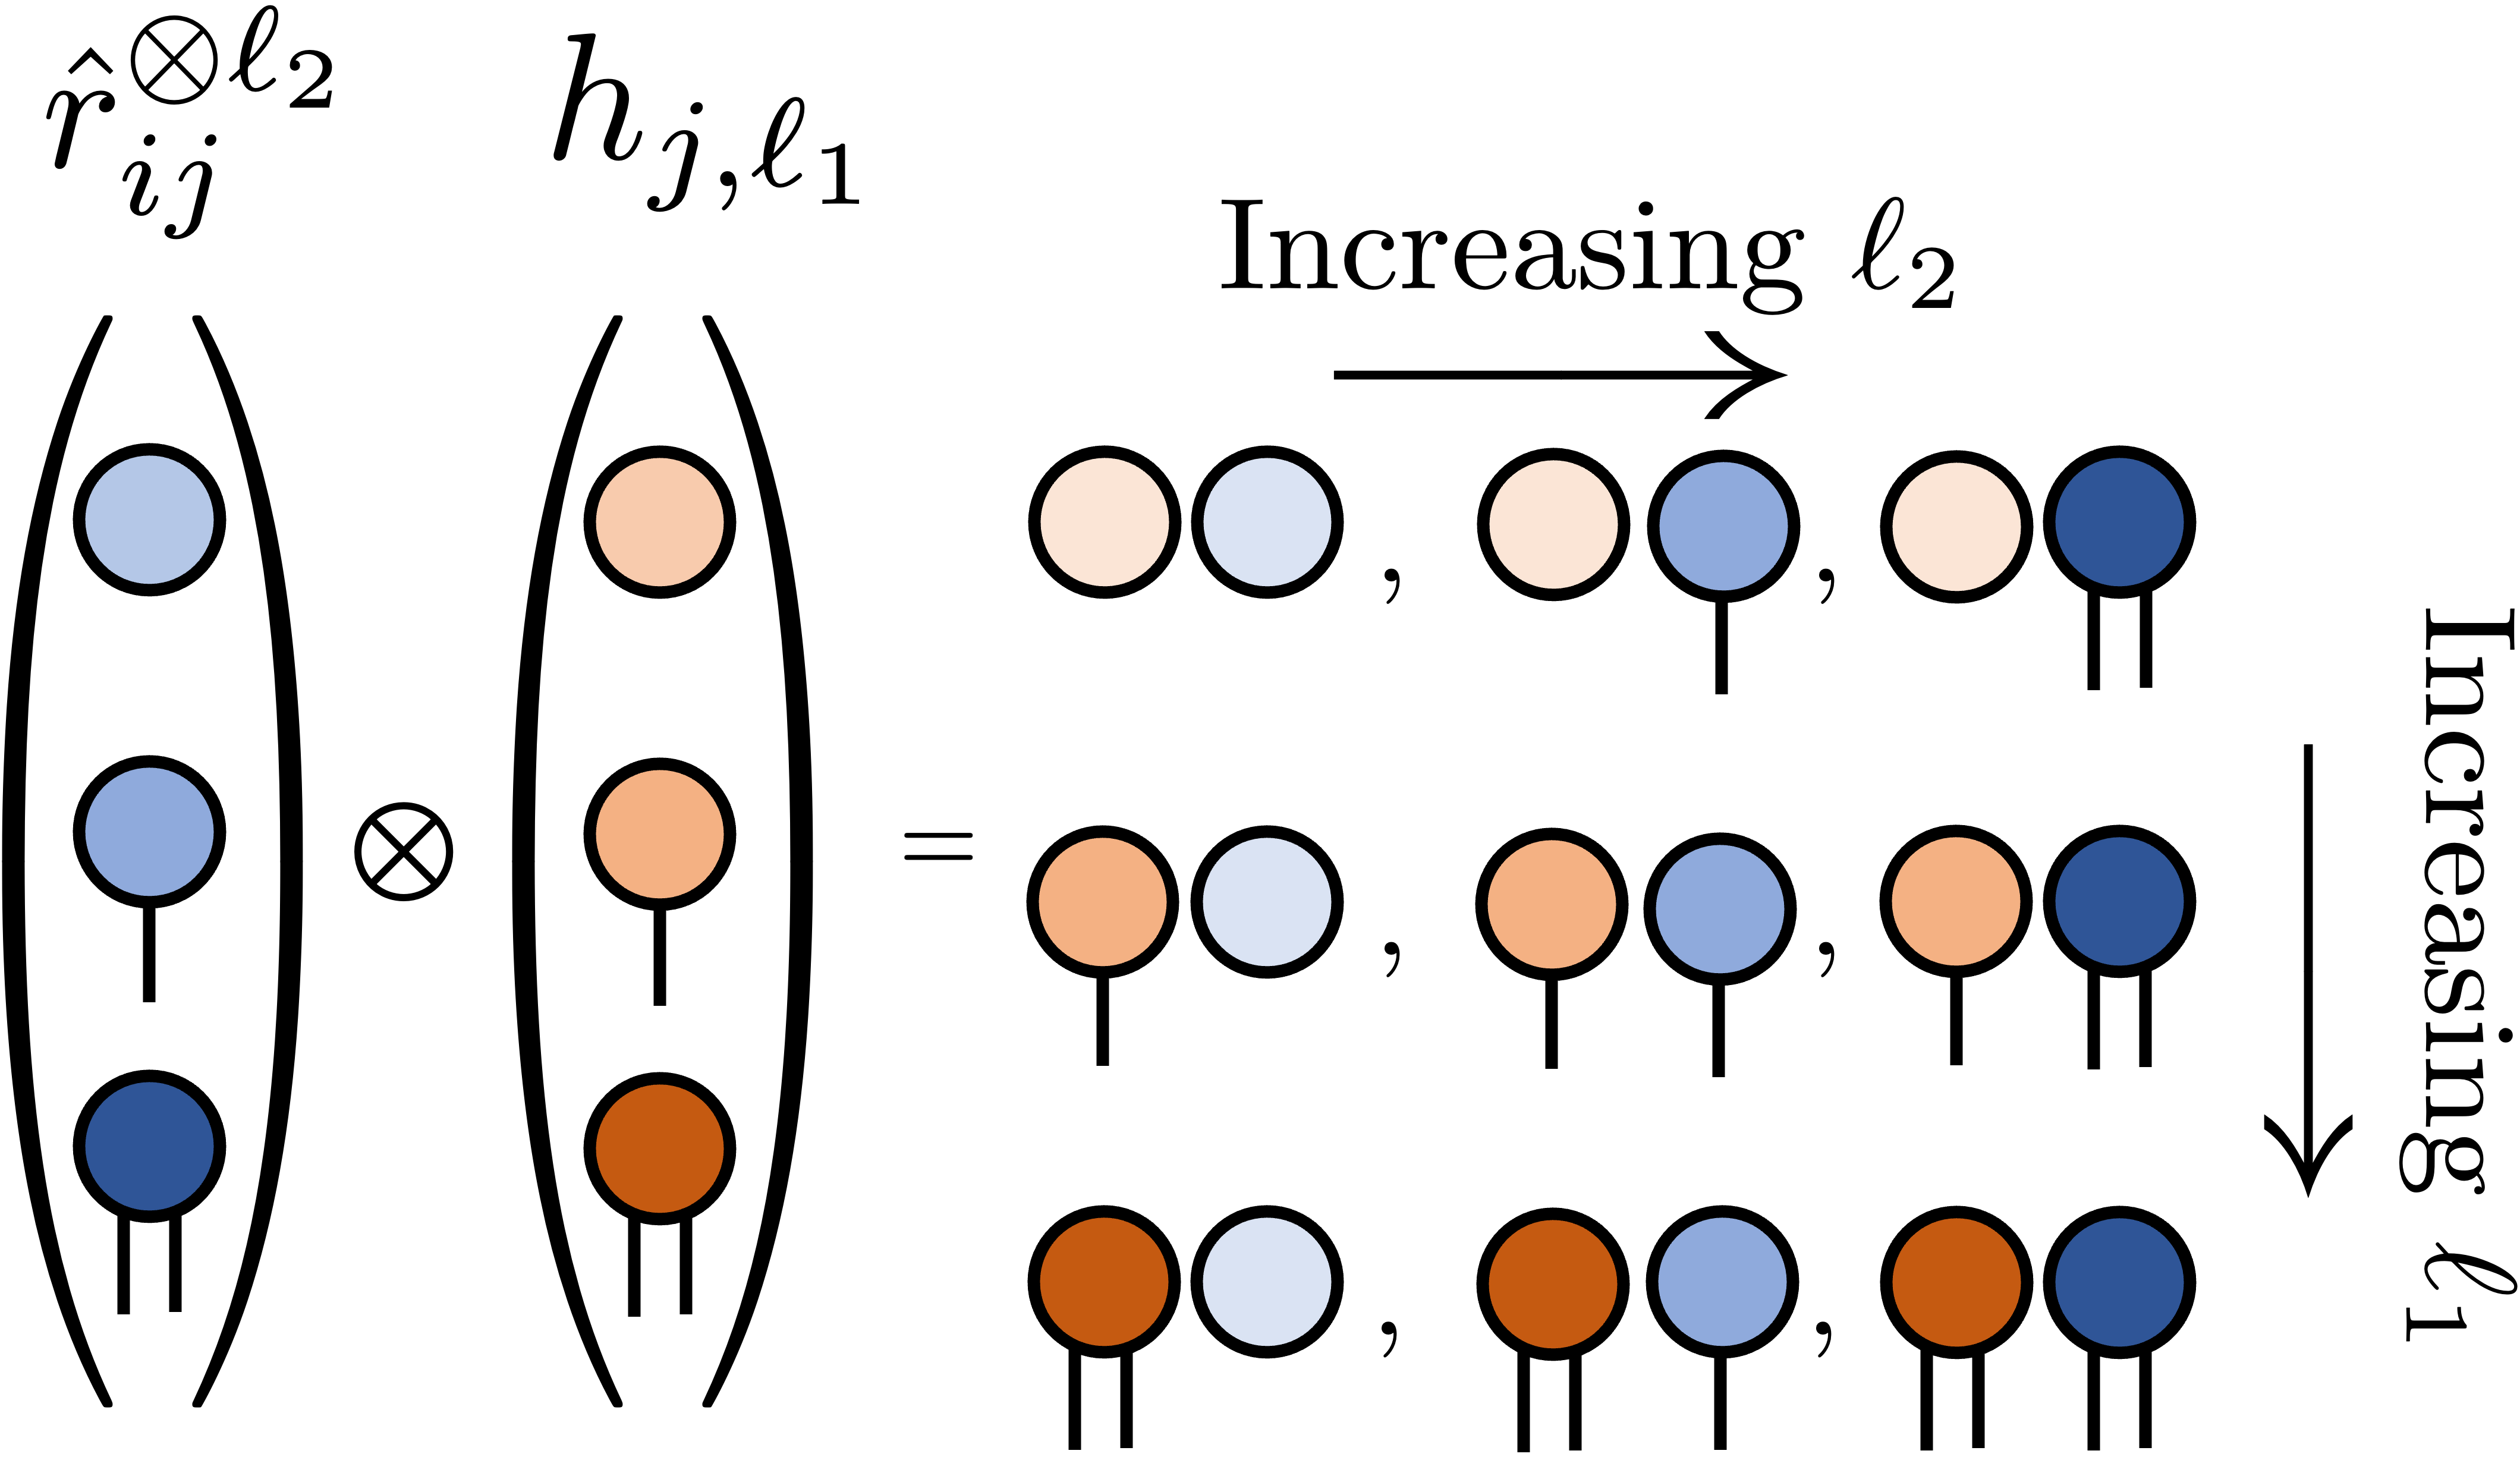
\includegraphics[scale=0.3]{figures/projection.png}
%     \caption{projection of the features tensors onto Cartesian tensors basis. Both of these have a maximum rank-$2$}
%     \label{fig:projection}
% \end{figure}

% \textbf{Contractions. } We can think of the tensor product between $\Theta$ and $h_j$ to be the projection of our features onto a set of basis tensors. Figure \ref{fig:projection} show this projection in the Cartesian basis, illustrating all possible tensor products of the basis tensors of rank $\ell_2$ and features tensors of rank $\ell_1$ for the case where they both have a maximum rank of $2$, we then multiply by the correct weighted RBF which is a scalar therefore doesn't affect the rank. The 9 output tensors can then be contracted into the desired output rank $\ell_3$ via the contract operator. All contractions to $\ell_3$ are them summed up. Therefore per edge we have one particle basis per tensor unique rank ($0 , 1, \cdots, \ell_{3,\text{3}}$)

% \subsection{Atomic Basis, $A$} 

% \begin{equation} \label{eq:atomic-basis}
%     A^{(t)}_{i,k\ell} = \sum_{j \in \mathcal N(i)} \phi_{j,k\ell}
% \end{equation}

% Formation of the atomic basis is a simple step in which we sum up the two-body particle basis states of each rank, $\phi_{ij, \ell_3}$ of node $i$ with all of its neighbours. This step leaves up with an atomic basis for each node.

% \subsection{Product Basis, $\mathbf{B}$}

% \begin{equation} \label{eq:prod}
%     \mathbf{B}^{(t)}_{i, \eta_\nu k L} = \underset{\sum_\xi \ell_\xi \rightarrow L}{\mathrm{contract}} \left( \bigotimes_{\xi=1}^{\nu} \underset{\ell_\xi}{\mathrm{mix}}(A^{(t)}_{i,k\ell_\xi}) \right)
% \end{equation}

% The formation of the product basis (equation \ref{eq:prod}) is the key step that allows for the implicit creation of higher body-order terms. The $B$'s for each node are formed out of only the atomic basis states from that same node (i.e. grows with the number of nodes!). The correlation order, $\nu$, gives us how many atomic basis tensors are used in constructing each $B$'s with that correlation order. The maximum implicit body order within a $B$ is $\nu + 1$. Figure \ref{fig:implicit-high-body} shows an example where we only consider scalar two-body particle states, with $\nu=2$, here we see that we have implicit three body terms. Any of these terms can be picked out of the sum as each two-body state have learned weights from the RBFs.  

% \begin{figure}[H]
%     \centering
%     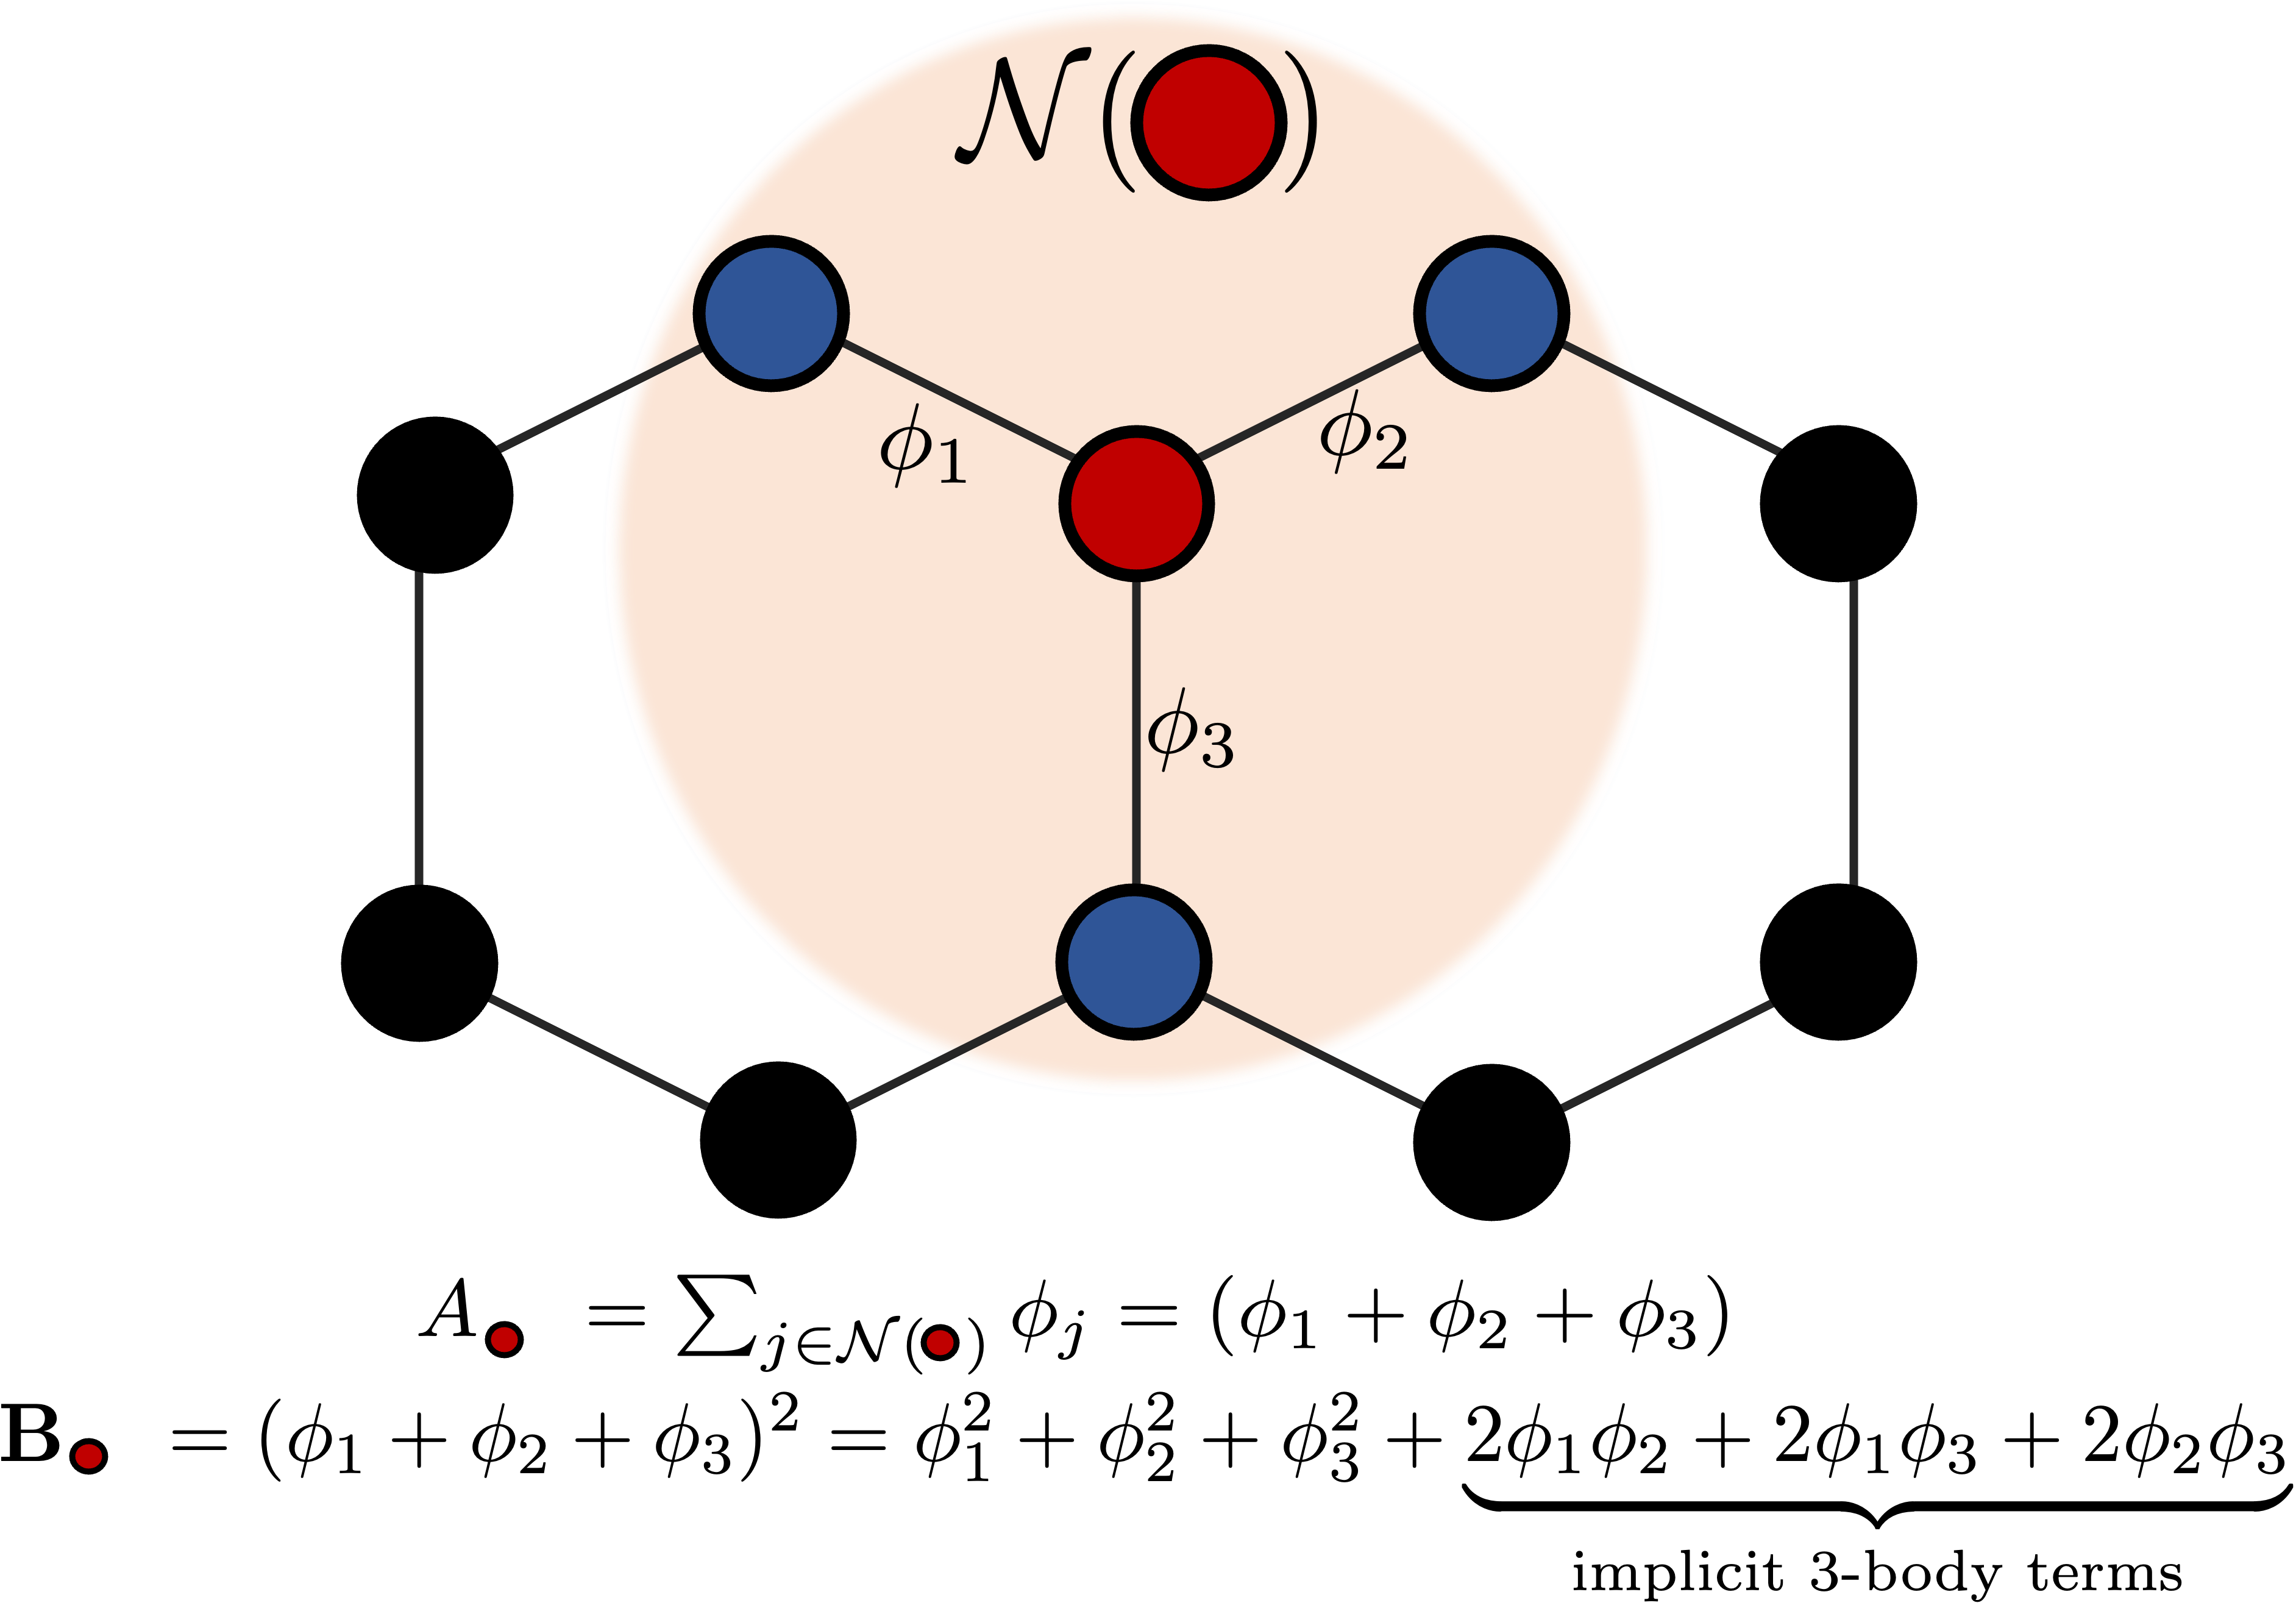
\includegraphics[scale=0.4]{figures/implicit-high-body.png}
%     \caption{MACE's benefit comes from the fact that we can implicitly extract higher body-order features at a fraction of the cost of enumerating explicitly}
%     \label{fig:implicit-high-body}
% \end{figure}

% For each $\nu$ we can pick from any of the $A$ states of that node (i.e. scalar, vector, matrix, ...) - we call each unique combination a split, which can be represented by the tuple $(\ell_1, \ell_2, \cdots, \ell_\nu)$. For example, if $\nu=2$ and the maximum rank of the atomic basis is $2$ we can have six different splits - $(0,0), (0,1), (0,2), (1,1), (1,2), (2,2)$. For each split the $A$'s chosen have their channels mixed (unique to this split). Finally, these tensor products of $A$ are contracted down from the tensor product rank (sum of element in the split tuple $\sum_\xi \ell_\xi$), down to the desired output rank $L$. The $\nu$ and split that a contraction originates from defines its path which is indexed by $\eta_\nu$ in $\mathbf{B}$.


% The computational speed of MACE comes from the fact that the architecture never explicitly calculates the tensor products in Equation \ref{eq:prod} as only contractions, that absorb the tensor product are ever required. 

% For example, if we have the tensors $A_{ijk}, B{lmn}$ and we want to perform a contraction over the indices $(i,l), (j,m), (k,n)$ of the tensor product of $A$ and $B$. We could calculate the tensor product and then sum over repeated indices or we could sum over repeated indices first and then compute the tensor product (probably talk about non-scalar output case for clarity. 

% \begin{equation}
%     \sum_{ijk} C_{ijkijk} = \sum_{ijk} A_{ijk} \otimes B_{ijk}
% \end{equation}


% in this example the first method need us to calculate and store a tensor with $3^6 = 729$ elements where as the second method need us to access two tensors that we are already storing each with $2 \times 3^3  = 54$ elements. It is easy to see that this scales exponentially so only becomes more important as our maximum rank of $A$ and our max correlation $\nu_\text{max}$ increases. We can think of it like sampling different low rank properties of the full rank tensor. These implicitly calculated tensors may have rank of upto 15, these tensors will be extremely expressive such that even the low-rank projections are very useful. As we are using learned weights, the most important low-rank properties i.e. $B$'s will becomes very important in the output. This idea is reminiscent of \textit{the kernel trick} in Support Vector Machines in which a high-dimensional space is implicitly accessed via inner products (contraction over a pair of vectors). **


% \subsection{The Message, $m$} 

% \begin{equation} \label{eq:message}
%     m_{i,L}^{(t)} =  \sum_{\nu} \sum_{\eta_{\nu}} W_{z_{i} L, \eta_{\nu}}^{(t)} B^{(t)}_{i,\eta_\nu L}
% \end{equation}

% The \textit{message} is formed via a (learned) linear combination of all the product basis states $B$ (by consdering all paths for all correlation order). Figure \ref{fig:create-message} illustrates what this message the scalar and vector message would look like in tensor network notation, with the highest rank representation of the atomic basis being matrices and the maximum correlation order being $4$, the different colours represent channel mixings. 

% \begin{figure}[H]
%     \centering
%     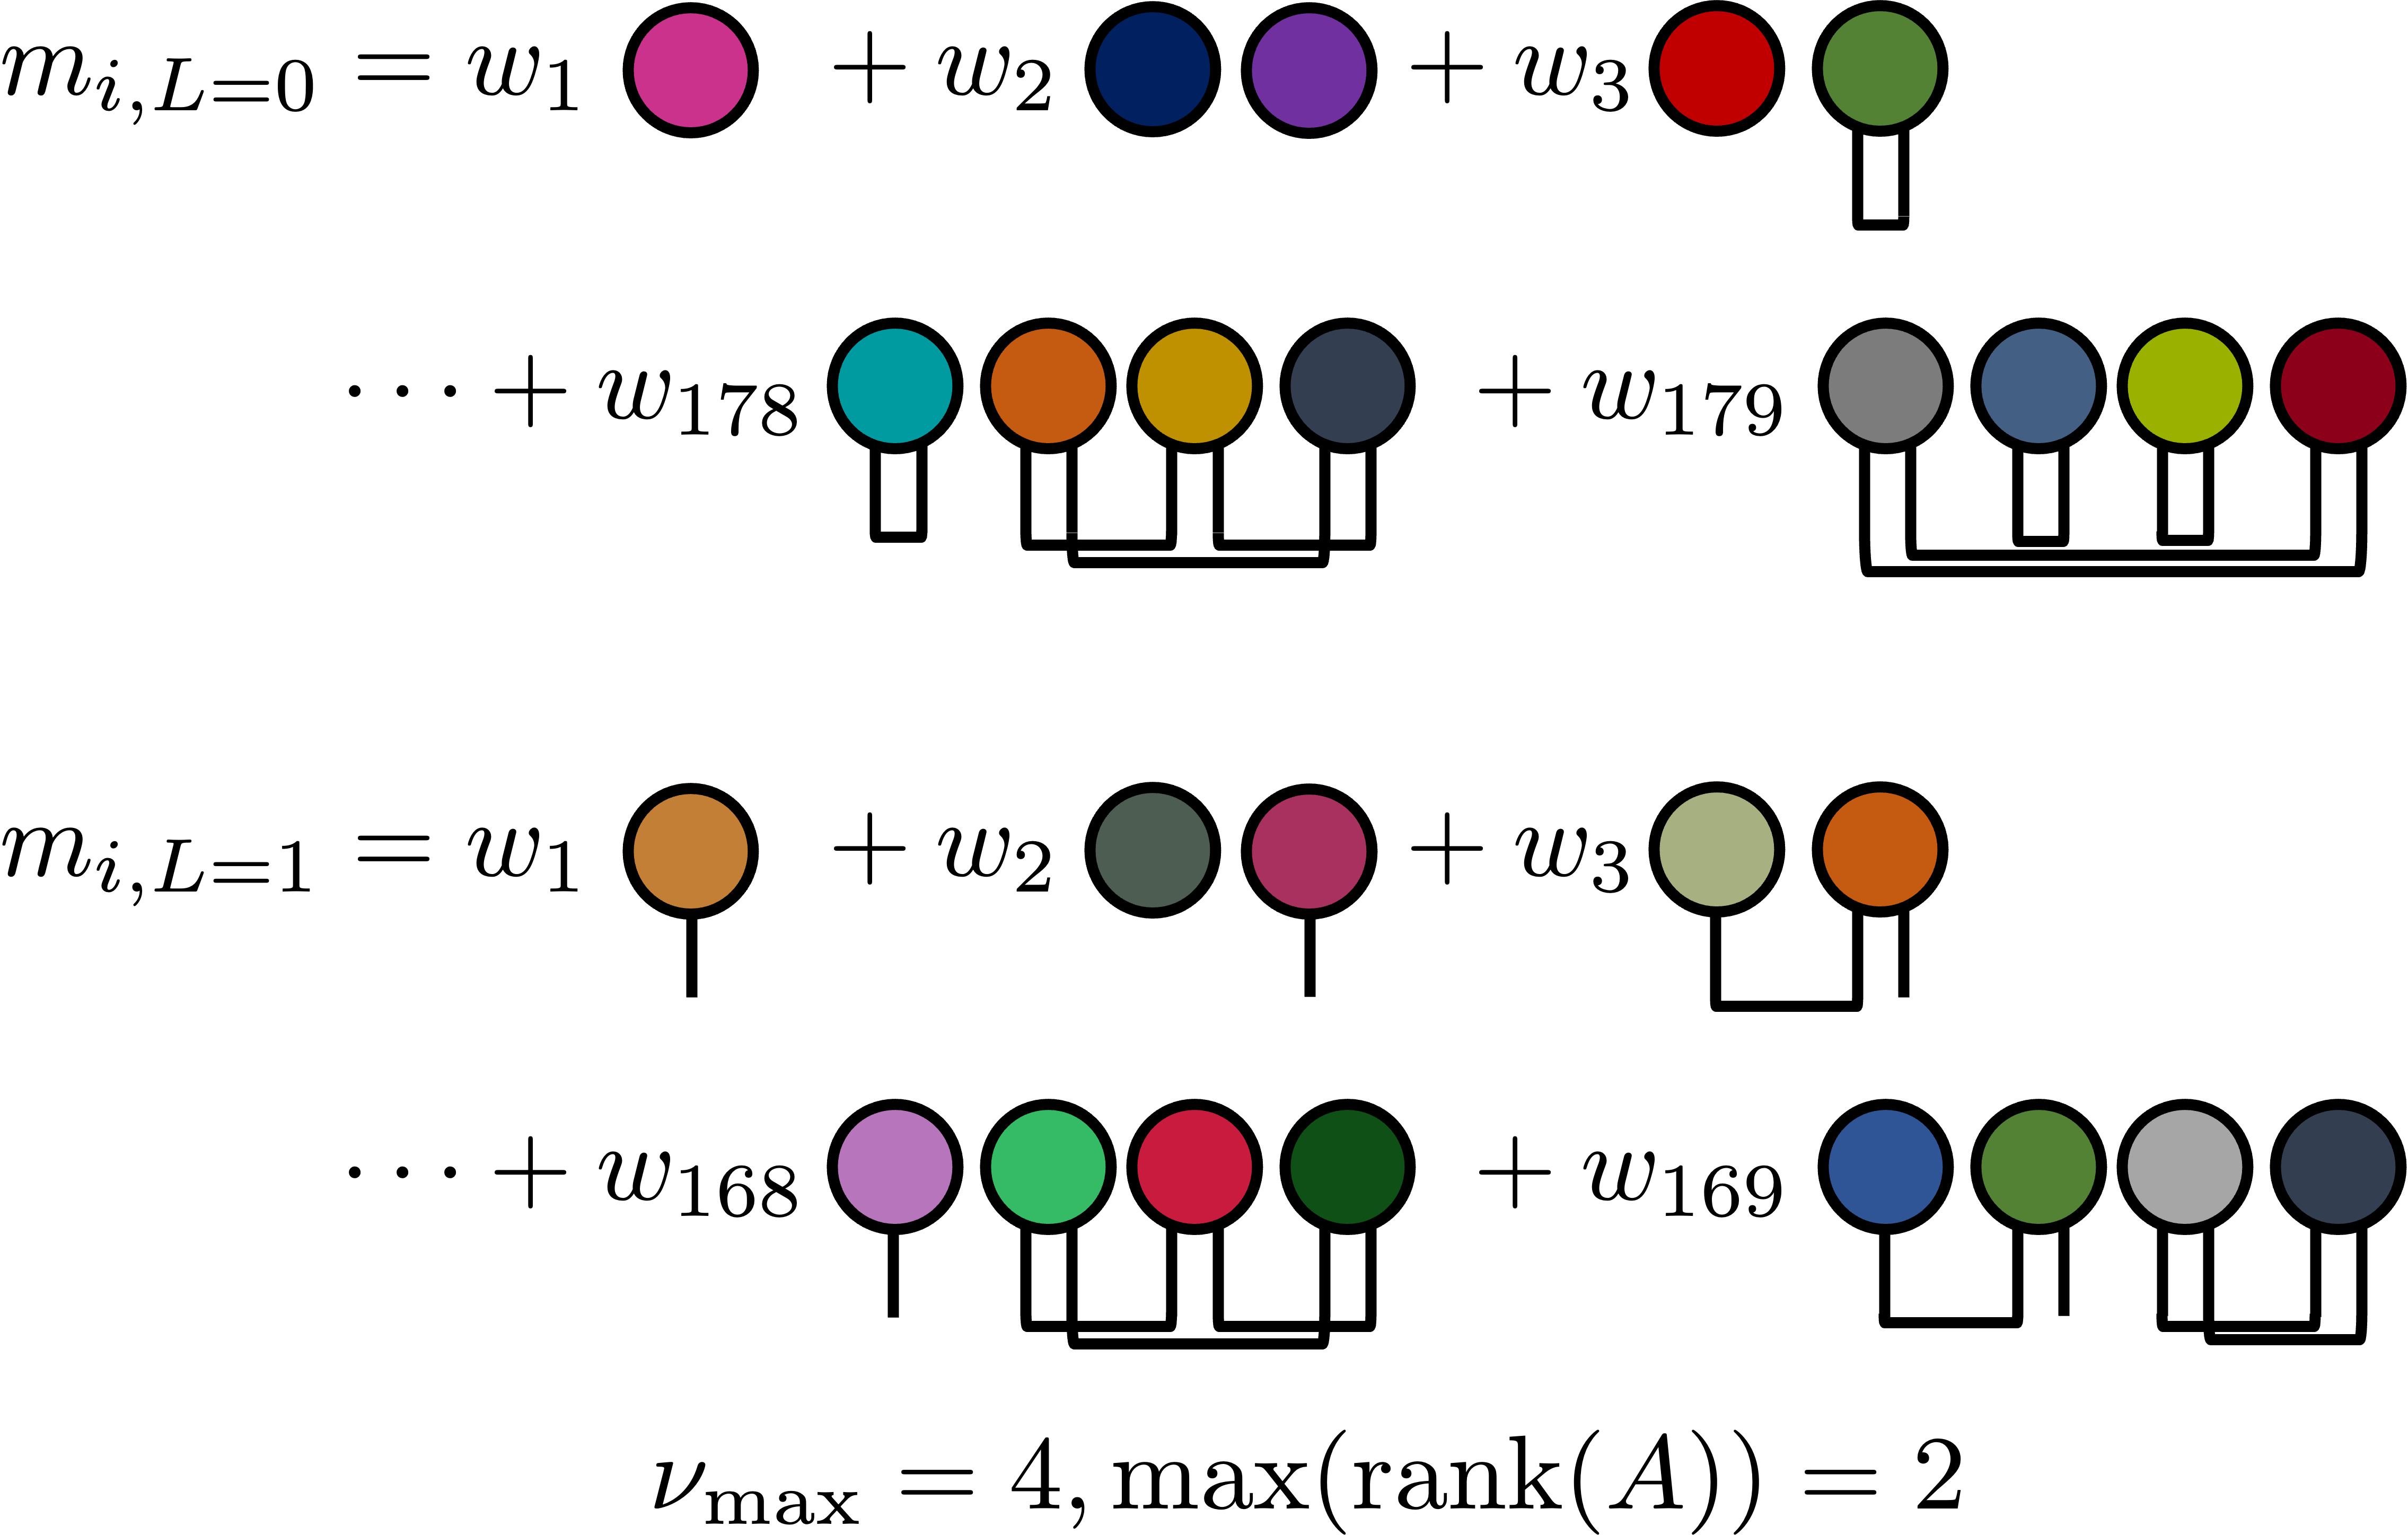
\includegraphics[scale=0.3]{figures/create-message.png}
%     \caption{Message creation by a weighted sum of all tensors contractions to the desired rank. Here we have two examples for $\nu_max=4$ and maximum atomic basis rank $=2$. Production of scalar and vector messages respectively}
%     \label{fig:create-message}
% \end{figure}


% \subsection{Updating Features} 
% Features are then updated via equation \ref{eq:update} in which the channels of the messages are mixed and are added together with the current features whose channels have also been mixed, this is called a residual connection \cite{he2016deep} which works under the basic principle that to prevent vanishing gradient we should use `skip' connections between layers.  

% \begin{equation} \label{eq:update}
%     h^{(t+1)}_{i,k L} = \mathrm{mix}(m^{(t)}_{i,k L})
%     + \mathrm{mix}(h^{(t)}_{i,kL})
% \end{equation}
